\chapter{Implementacja aplikacji}
W niniejszym rozdziale znajduje się opis struktur danych znajdujących się w bazach danych.
Opisane interfejsy programistyczne, modeli danych oraz zasady działania części serwerowej.
Przedstawione widoki interfejsu użytkownika. Zostały opisane zasady współpracy serwera i aplikacji mobilnej.
%
\section{Model bazy danych}
W systemie wykorzystano dwie nierelacyjne bazy danych: MongoDB i Redis.
MongoDB jest przeznaczona do przechowywania danych aplikacji.
Redis wykorzystuje się tylko do czasowego przechowywania tokenów.

% 
\paragraph{MongoDB\newline}
% TO DO: proszę stosować czcionkę maszynową do kodu źródłowego, nazw zmiennych i klas, nazw plików itp.
% DONE: dziękuję, po prostu nie wiedziałem jak to zrobić z nazwami.
% TO DO: aby zdefiniować zawartość plików json można posłużyć się specyfikacją json schema : https://json-schema.org/
% TO DO: prawdopodobnie dokumenty w MongoDB powstają poprzez mapowanie z obiektów dostępnych w języku programowania,
%  jeśli tak jest, to należy o tym powiedzieć (w opisie implementacji można pokazać diagram klas zawierających odpowiednie pola)
% TO VERIFY: ten json jest wycinkiem z konsoli bazy danych ,,mongo'' po wprowadzeniu odpowiedniego zapytania (,,db.nazwakolekcji.find({});''), różni się od odpowiedzi, które otrzymałem w tej konsoli tym, że sformatowano do czytelnego tekstu, a nie wszystko w jednej linii.
Baza danych składa się z dwóch kolekcji: \texttt{station} i \texttt{user}. Kolekcja \texttt{user} składa się z następujących pól:
\texttt{
    \begin{itemize}
        \item \_id : ObjectId(String)
        \item user\_name : String
        \item email : String
        \item password : String
        \item Model : Object :
        \begin{itemize}
            \item create\_at : ISODate
            \item update\_at : ISODate
            \item delete\_at : ISODate
        \end{itemize}
    \end{itemize}
}

Przykład encji:
\begin{lstlisting}[basicstyle=\tiny\ttfamily]
    {
        "_id":ObjectId("5fb93e4b721953b7c60983c6"),
        "user_name":"newtest",
        "email":"newtest@test.test",
        "password":"$2a$04$o0WfZvdk4WUpsct.BH3zw.3MFJFmUuLe8VjJx2OeyxtZuBliMOrl.",
        "model":{
            "create_at":ISODate("2020-11-21T16:20:27.044Z"),
            "update_at":ISODate("2020-11-21T16:20:27.044Z"),
            "delete_at":ISODate("0001-00-00T00:00:00Z")
        }
    }
\end{lstlisting}

Kolekcja \texttt{station} składa się z następujących pól:
\texttt{
    \begin{itemize}
        \item \_id : String
        \item station\_name : String
        \item owner\_id : String
        \item rating : Double
        \item latitude : Double
        \item longitude : Double
        \item description : String
        \item comments : Array :
        \begin{itemize}
            \item \_id : String
            \item user\_id : String
            \item user\_name : String
            \item text : String
            \item rating : Double
            \item model : Object :
            \begin{itemize}
                \item create\_at : ISODate
                \item update\_at : ISODate
                \item delete\_at : ISODate
            \end{itemize}
        \end{itemize}
        \item model : Object :
        \begin{itemize}
            \item create\_at : ISODate
            \item update\_at : ISODate
            \item delete\_at : ISODate
        \end{itemize}
    \end{itemize}
}

Przykład encji:
\begin{lstlisting}[basicstyle=\tiny\ttfamily]
    {
        "_id":ObjectId("5fca6f81bb37f04ad438c1a5"),
        "station_name":"Station Name",
        "owner_id":"5fb828babe10c57ba70d49cd",
        "rating":3.6666666666666665,
        "description":"description",
        "latitude":57.12662933894774,
        "longitude":14.208925142884254,
        "model":{
            "create_at":ISODate("2020-12-04T17:18:57Z"),
            "update_at":ISODate("2020-12-04T17:20:55Z"),
            "delete_at":ISODate("0001-00-00T00:00:00Z")
        },
        "comments":[
            {
                "_id":"5fca6ff7bb37f04ad438c1a8",
                "user_id":"5fb828babe10c57ba70d49cd",
                "user_name":"test",
                "text":"  Comment 3",
                "rating":5,
                "model":{
                    "create_at":ISODate("2020-12-04T17:20:55Z"),
                    "update_at":ISODate("2020-12-04T17:20:55Z"),
                    "delete_at":ISODate("0001-00-00T00:00:00Z")
                }
            },
            {
                "_id":"5fca6fe5bb37f04ad438c1a7",
                "user_id":"5fb828babe10c57ba70d49cd",
                "user_name":"test",
                "text":" Comment 2",
                "rating":3,
                "model":{
                    "create_at":ISODate("2020-12-04T17:20:37Z"),
                    "update_at":ISODate("2020-12-04T17:20:37Z"),
                    "delete_at":ISODate("0001-00-00T00:00:00Z")
                }
            },
            {
                "_id":"5fca6fb8bb37f04ad438c1a6",
                "user_id":"5fb828babe10c57ba70d49cd",
                "user_name":"test",
                "text":"Comment 1",
                "rating":3,
                "model":{
                    "create_at":ISODate("2020-12-04T17:19:52Z"),
                    "update_at":ISODate("2020-12-04T17:19:52Z"),
                    "delete_at":ISODate("0001-00-00T00:00:00Z")
                }
            }
        ]
    }
\end{lstlisting}

% 
\paragraph{Redis\newline}
Baza danych Redis wykorzystana tylko dla przechowywania tokenów użytkowników, które już wylogowane, ponieważ jedną z wad JWT tokenów jest to, że wygenerowany token nie można określić jako niedziałający, dopóki nie skończy się określony czas jego działania.
Redis częściowo eliminuje ten problem.

W nim przechowuje się para ,,klucz - wartość'', pewny czas. Po upływie tego czasu zapis automatycznie jest usuwany.
Dla szybkiego wyszukiwania encja wygląda w następujący sposób: \texttt{token}, \texttt{token}. To pozwala często wylogować się użytkownikowi, ale zajmuje więcej miejsca niż encja typu: \texttt{user\_id}, \texttt{token}.

\section{Implementacja części serwerowej}
% 
\subsection{Struktura RestApi}
% 
\subsubsection{Narzędzia, technologie, biblioteki}
Do stworzenia serwerowej części aplikacji użyto następujących technologii:
\begin{itemize}
\item Visual Studio Code - środowisko programistyczne;
\item Go - język programowania;
\item Go Modules - system zarządzania zależnościami;
\item gorilla/mux - Router mapuje przychodzące żądania na listę zarejestrowanych tras i wywołuje moduł obsługi tego żądania, który odpowiada URL (ang. \textit{Uniform Resource Locator}) adresowi;
\item sirupsen/logrus - rejestrator strukturalny;
\item mongo-driver - sterowanie MongoDB z języka Go;
\item go-redis/redis - sterowanie Redis z języka Go;
\item dgrijalva/jwt-go - realizacja JWT w języku Go;
\item crypto/bcrypt - realizuje algorytm haszowania bcrypt;
\item go-ozzo/ozzo-validation - pakiet wspomagający na walidację danych;
\item yaml.v2 - implementuje obsługę YAML (ang. \textit{Yet Another Markup Language});
\item google/uuid - sprawdza i generuje UUID (ang. \textit{universally unique identifier});
\end{itemize}

% 
\subsubsection{Struktura plików RestApi}
Na rysunku \ref{fig:backend_file_structure} została przedstawiona struktura plików części serwerowej. Obok plików, niezbędnych do działania aplikacji, znajdują się pliki pozwalające na prowadzenie testów jednostkowych. Te pliki mają nazwę w postaci \texttt{*\_test.go}.
% TO DO: proszę poukładać obrazki ze strukturami plików obok siebie (pojedynczo zajmują za dużo miejsca)
% TO VERIFY:
\begin{figure}[ht]
\centering
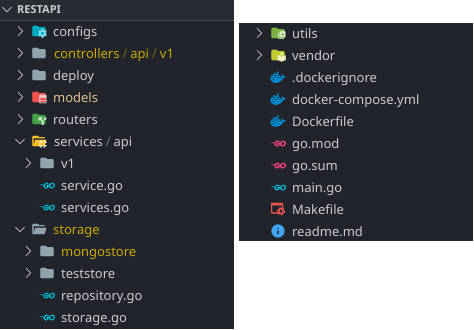
\includegraphics[width=0.25\linewidth]{rys03/backend_file_structure.png}
\caption{Struktura plików}
\label{fig:backend_file_structure}
\end{figure}
\begin{figure}[ht]
	\centering
    \begin{tabular}{@{}rl@{\hspace{3mm}}rl@{\hspace{3mm}}rl@{}}
        a) & \vtop{\vskip-2ex\hbox{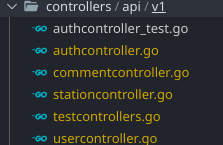
\includegraphics[width=0.25\linewidth]{rys03/controllers.png}}} &
        b) & \vtop{\vskip-2ex\hbox{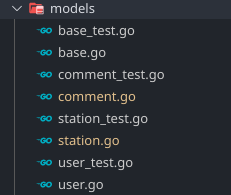
\includegraphics[width=0.25\linewidth]{rys03/model.png}}} &
        c) & \vtop{\vskip-2ex\hbox{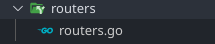
\includegraphics[width=0.25\linewidth]{rys03/routers.png}}}
    \end{tabular}
    \caption{Struktura plików: a) kontrolery, b) modeli danych, c) routery.}
    \label{fig:backend_file_structure_1}
\end{figure}
\begin{figure}[ht]
	\centering
    \begin{tabular}{@{}rl@{\hspace{3mm}}rl@{\hspace{3mm}}rl@{}}
        a) & \vtop{\vskip-2ex\hbox{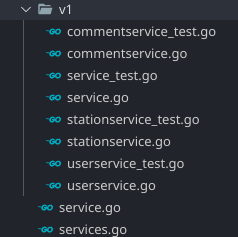
\includegraphics[width=0.25\linewidth]{rys03/services.png}}} &
        b) & \vtop{\vskip-2ex\hbox{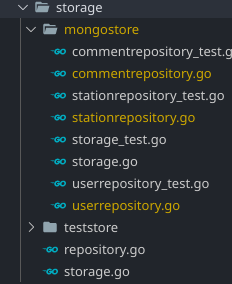
\includegraphics[width=0.25\linewidth]{rys03/storage.png}}} &
        c) & \vtop{\vskip-2ex\hbox{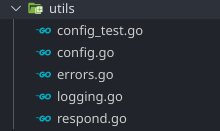
\includegraphics[width=0.25\linewidth]{rys03/utils.png}}}
    \end{tabular}
    \caption{Struktura plików: a) serwisy, b) wszpółdziałania z bazą danych, c) narzędzia.}
    \label{fig:backend_file_structure_2}
\end{figure}

Katalog \texttt{config} zawiera pliki konfiguracyjne.

W katalogu \texttt{controllers} (rys.~\ref{fig:backend_file_structure_1}a) znajdują się kontrolery, które służą do kontrolowania zapytania, opracowania i zwrotu danych. Warstwa Kontrolerów komunikuje z warstwą serwisów,

Do katalogu \texttt{deploy} jest kompilowana aplikacja przy uruchomieniu \texttt{Makefile}.

Katalog \texttt{models}(rys. \ref{fig:backend_file_structure_1}b) zawiera modeli danych.

Katalog \texttt{routers} (rys. \ref{fig:backend_file_structure_1}c) zawiera plik, w którym są definiowane punkty końcowe (ang.~\emph{endpoints}) części serwerowej oraz zachodzi ich mapowanie na kontrolery.

Funkcje lub metody przechowywane w katalogu \texttt{services} (rys. \ref{fig:backend_file_structure_2}a) prowadzą biznes logikę (obróbkę danych i podejmują decyzję co z nimi trzeba zrobić). Warstwa serwisów komunikuje z warstwą \texttt{DAL} (ang. \textit{data access layer}). Część tych metod nie mają logiki biznesowej, natomiast one zaimplementowane w celu ułatwiania rozszerzenia funkcjalności, do podtrzymywania porządku w aplikacji oraz zgodności z Rest API architekturą.

Współpraca z bazą danych zachodzi w katalogu \texttt{storage} (rys. \ref{fig:backend_file_structure_2}b). Jest to warstwa \texttt{DAL} która przeznaczona do komunikacji z bazą danych. Katalog \texttt{mongostore} współdziała z MongoDB, natomiast \texttt{teststore} wykorzystuje się do testowania, które będzie omówione w rozdziale \ref{ch:Testy}.

W katalogu \texttt{utils} (rys. \ref{fig:backend_file_structure_2}c) znajdują się rzeczy wspomagające, na przykład lista błędów lub rejestracja działania serwera.

\subsubsection{Konfiguracja serwera}
Do zapobiegania ponownie kompilacji w przypadku zmiany portu, na którym działa serwer lub adresów baz danych, została utworzona struktura \texttt{Config} \ref{list:config_restapi} (plik utils/config.go), która przy uruchomieniu aplikacji pobiera dane z pliku, który zostanie podany jako parametr wejściowy.
Plik musi być typu \texttt{yaml}. Za pomocą biblioteki \texttt{yaml.v2} ten plik jest parsowany do obiektu struktury \texttt{Config} \ref{list:config_restapi_new}. Przykład pliku:\begin{lstlisting}[basicstyle=\tiny\ttfamily]
    bind_addr: :8081
    database_url: mongodb://127.0.0.1:27017
    db_name: elCharge
    db_user_collection: user
    db_station_collection: station
    db_redis: 127.0.0.1:6379
    jwtKey: 21d5680b6a
\end{lstlisting}

\begin{lstlisting}[label=list:config_restapi,caption=Klasa konfiguracyjna części serwerowej,basicstyle=\tiny\ttfamily]
    type Config struct {
        BindAddr            string `yaml:"bind_addr"`
        DatabaseURL         string `yaml:"database_url"`
        DbName              string `yaml:"db_name"`
        DbUserCollection    string `yaml:"db_user_collection"`
        DbStationCollection string `yaml:"db_station_collection"`
        RedisDB             string `yaml:"db_redis"`
        JWTKey              string `yaml:"jwtKey"`
    }
\end{lstlisting}

\begin{lstlisting}[label=list:config_restapi_new,caption=Wczytanie pliku konfiguracyjnego części serwerowej,basicstyle=\tiny\ttfamily]
    func NewConfig(path string) (*Config, error) {
        configFile, err := ioutil.ReadFile(path)
        if err != nil {
            return nil, err
        }
        config := &Config{}
        err = yaml.Unmarshal(configFile, config)
        if err != nil {
            return nil, err
        }
        return config, nil
    }
\end{lstlisting}
% 
\subsubsection{Przepływ danych}
Na rysunku \ref{fig:backend_data_flow} został przedstawiony schemat przetwarzania i przepływu danych przy wysyłaniu zapytania do części serwerowej niniejszej aplikacji.
% TO DO: rysunek do przerysowania (proszę zacieśnić bloczki, wtedy przy skalowaniu do szerokości strony czcionka stanie się większa
% DONE:
\begin{figure}[ht]
\centering
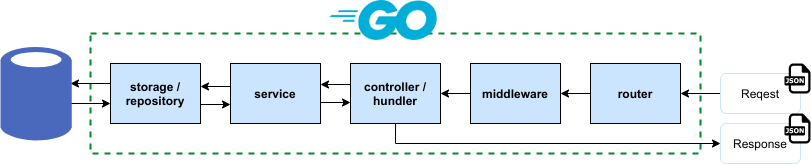
\includegraphics[width=1\linewidth]{rys03/backend_data_flow.png}
\caption{Przepływ danych}
\label{fig:backend_data_flow}
\end{figure}

% 
\subsubsection{Punkty końcowe}
Część serwerowa jest napisana zgodnie z modelem Rest API. Wymiana danymi zachodzi za pomocą standardów: HTTP (ang. \textit{HyperText Transfer Protocol}), URL, JSON.
W tabeli \ref{tab:endpoints} przedstawiony spis endpointów razem z metodą ich wysłania oraz krótkim opisem.
\begin{table}[htb] \small
    \caption{Lista Enpointów części serwerowej}
    \label{tab:endpoints}
    \begin{tabularx}{\linewidth}{| m{0.45cm} | m{1.5cm} | m{6cm} | X |}
    \hline
    № & Metoda & Endpoint & Opis \\
    \hline
    1 & GET & /api/v1 & Endpoint do testowania działania serwera. \\
    \hline
    2 & POST & /api/v1/login & Zalogowanie się użytkownika. \\
    \hline
    3 & GET & /api/v1/logout & Wylogowanie się użytkownika. \\
    \hline
    4 & POST & /api/v1/users & Tworzenie użytkownika / rejestracja \\
    \hline
    5 & GET & /api/v1/users/{id} & Wczytywanie danych jednego użytkownika. \\
    \hline
    6 & PUT & /api/v1/users/{id} & Edycja użytkownika. \\
    \hline
    7 & DELETE & /api/v1/users/{id} & Usuwanie użytkownika. \\
    \hline
    8 & GET & /api/v1/users/read?skip=""\&limit="" & Wczytywanie danych limitowanej listy użytkowników użytkownika. \\
    \hline
    9 & POST & /api/v1/stations & Tworzenie stacji ładowania. \\
    \hline
    10 & GET & /api/v1/stations/{id} & Wczytywanie danych jednej stacji ładowania. \\
    \hline
    11 & PUT & /api/v1/stations/{id}?ownid="" & Edycja stacji. \\
    \hline
    12 & DELETE & /api/v1/stations/{id}?ownid="" & Usuwanie stacji ładowania. \\
    \hline
    13 & GET & /api/v1/stations/read?skip=""\&limit=""\&lat=""\&lng=""\&dist=""\&descr=""\&nam="" & Wyszukiwnaie stacji ładowania w zależności od parametrów. \\
    \hline
    14 & POST & /api/v1/stations/\{sid\}/comments & Tworzenie komentarza. \\
    \hline
    15 & GET & /api/v1/stations/\{sid\}/comments{id} & Wczytywanie danych jednego komentarza. \\
    \hline
    16 & PUT & /api/v1/stations/\{sid\}/comments{id} & Edycja komentarza. \\
    \hline
    17 & DELETE & /api/v1/stations/\{sid\}/comments{id} & Usuwanie komentarza. \\
    \hline
    18 & GET & /api/v1/stations/\{sid\}/read?skip=""\&limit="" & Wczytywanie danych limitowanej listy komentarzy należących do pewnej stacji. \\
    \hline
    \end{tabularx}
\end{table}

Kodem \ref{list:routers} została przedstawiona implementacja endpointów.
Dla rejestracji połączeń wchodzących zostały użyte metody medialne: \texttt{s.logger.SetRequestID}, do przeznaczenia id każdemu połączeniu ,oraz \texttt{s.logger.LogRequest}, do wypisywania tego do konsoli.
Dla większości przypadków też jest sprawdzano czy jest użytkownik zalogowany do systemu \texttt{s.authController.CheckToken}. To będzie wyjaśnione później (sekcja \ref{sec:autentykacja}).
\begin{lstlisting}[label=list:routers,caption=Implementacja punktów końcowych,basicstyle=\tiny\ttfamily]
    func (s *Server) SetupRouters() *mux.Router {
        v1 := "/api/v1"
        s.router.Schemes("http")
        s.router.Use(s.logger.SetRequestID) // middleware
        s.router.Use(s.logger.LogRequest)   // middleware
        s.router.HandleFunc(v1, s.testController.TestAPIV1()).Methods("GET")
        s.router.HandleFunc(v1+"/users", s.authController.CreateUser()).Methods("POST")
        s.router.HandleFunc(v1+"/login", s.authController.Login()).Methods("POST")
        s.router.HandleFunc(v1+"/logout/{id}", s.authController.Logout()).Methods("GET")

        user := s.router.PathPrefix(v1 + "/users").Subrouter()
        user.Use(s.authController.CheckToken)
        user.HandleFunc("/read", s.userController.Read()).Methods("GET")
        user.HandleFunc("/{id}", s.userController.FindByID()).Methods("GET")
        user.HandleFunc("/{id}", s.userController.DeleteByID()).Methods("DELETE")
        user.HandleFunc("/{id}", s.userController.UpdateByID()).Methods("PUT")

        stat := s.router.PathPrefix(v1 + "/stations").Subrouter()
        stat.Use(s.authController.CheckToken)
        stat.HandleFunc("", s.statController.CreateStation()).Methods("POST")
        stat.HandleFunc("/read", s.statController.Read()).Methods("GET")
        stat.HandleFunc("/{id}", s.statController.FindByID()).Methods("GET")
        stat.HandleFunc("/{id}", s.statController.DeleteByID()).Methods("DELETE")
        stat.HandleFunc("/{id}", s.statController.UpdateByID()).Methods("PUT")

        comm := stat.PathPrefix("/\{sid\}/comments").Subrouter()
        comm.Use(s.authController.CheckToken)
        comm.HandleFunc("/read", s.commController.Read()).Methods("GET")
        comm.HandleFunc("", s.commController.CreateComment()).Methods("POST")
        comm.HandleFunc("/{id}", s.commController.FindByID()).Methods("GET")
        comm.HandleFunc("/{id}", s.commController.DeleteByID()).Methods("DELETE")
        comm.HandleFunc("/{id}", s.commController.UpdateByID()).Methods("PUT")
        return s.router
    }
\end{lstlisting}

% 
\subsection{Funkcje części serwerowej}
W tej sekcji są opisane implementacje endpointów części serwerowej.
% 
\subsubsection{Użytkownik}
Użytkownik jest niezbędny w pierwszej kolejności do uwierzytelniania. Niektóre dane użytkownika też są używane do rozumienia do kogo należy stacja ładownicza lub komentarz.

W listingu \ref{list:user_model} jest przedstawiona struktura użytkownika, wraz ze sposobem konwersji do JSON i BSON, która znajdująca się w pliku \texttt{models/user}.
\begin{lstlisting}[label=list:user_model,caption=Model danych użytkownika,basicstyle=\tiny\ttfamily]
    type User struct {
        ID       string `bson:"_id,omitempty" json:"_id,omitempty"`
        UserName string `bson:"user_name,omitempty" json:"user_name,omitempty"`
        Email    string `bson:"email,omitempty" json:"email,omitempty"`
        Password string `bson:"password,omitempty" json:"password,omitempty"`
        Model
    }
\end{lstlisting}

% 
% \paragraph{Dodawanie}\mbox{}\\
% Do tworzenia użytkownika został zaimplementowany endpoint \texttt{/api/v1/users}.
% Metoda zapytania \texttt{POST}.
% Jako ciało zapytania należy wysyłać obiekt w formacie JSON. Przykład:
% \begin{lstlisting}[basicstyle=\tiny\ttfamily]
%     {
%         "email": "email@test3.com",
%         "user_name": "test_user_1",
%         "password": "password"
%     }
% \end{lstlisting}
% Na serwerze nie sprawdza się, czy jest użytkownik już zalogowany, ponieważ ten endpoint również używany przy rejestracji.
% Zwraca JSON obiekt stworzonego użytkownika.

% Za pomocą routera jest realizowane przekierowanie z URL do wywołania metody kontrolera \texttt{CreateUser()} (listing \ref{list:user_controller_create}), w którym zaczyna się obróbka biznesowa zapytania.
% W tej metodzie są dekodowane dane z ciała zapytania, które są w formacie JSON, i przekazane do metody serwisu \texttt{CreateUser()} (listing \ref{list:user_service_create}). Po otrzymaniu danych z serwisu jest wysyłana odpowiedź.
% \begin{lstlisting}[label=list:user_controller_create,caption=Kontroler tworzenia użytkownika,basicstyle=\tiny\ttfamily]
%     func (c *UserController) CreateUser() http.HandlerFunc {
%         return http.HandlerFunc(func(w http.ResponseWriter, r *http.Request) {
%             u := &models.User{}
%             err := json.NewDecoder(r.Body).Decode(u)
%             if err != nil {
%                 utils.Error(w, r, http.StatusBadRequest, err)
%                 return
%             }
%             u, err = c.service.User().CreateUser(u)
%             if err != nil {
%                 utils.Error(w, r, http.StatusBadRequest, err)
%                 return
%             }
%             utils.Respond(w, r, http.StatusCreated, u)
%         })
%     }
% \end{lstlisting}

% W metodzie \texttt{CreateUser()} (listing \ref{list:user_service_create}) zachodzi:
% \begin{itemize}
%     \item walidacja danych;
%     \item sprawdzanie, czy istnieje użytkownik z taką pocztą mailową;
%     \item jeśli nie istnieje, to zachodzi szyfrowanie hasła oraz ustalenie czasu tworzenia i edycji obiektu. Jeśli już istnieje, to zwraca błąd;
%     \item tworzenie nowego użytkownika w bazie danych;
%     \item przygotowanie obiektu użytkownika do transmisji: usuwanie hasła i daty tworzenia dla bezpieczeństwa oraz szybkości transmisji danych.
% \end{itemize}
% Ta metoda znajduje się w pliku \texttt{services/v1/userservice.go}.
% \begin{lstlisting}[label=list:user_service_create,caption=Serwis tworzenia użytkownika,basicstyle=\tiny\ttfamily]
%     func (s *UserService) CreateUser(u *models.User) (*models.User, error) {
%         if err := u.Validate(); err != nil {
%             return u, err
%         }
%         _, err := s.storage.User().FindByEmail(u.Email)
%         if err != utils.ErrRecordNotFound {
%             if err != nil {
%                 return nil, err
%             }
%             return u, utils.ErrRecordAlreadyExists
%         }
%         if err := u.BeforeCreate(); err != nil {
%             return u, err
%         }
%         id, err := s.storage.User().Create(u)
%         if err != nil {
%             return nil, err
%         }
%         u, err = s.storage.User().FindByID(id)
%         if err != nil {
%             return nil, err
%         }
%         u.Sanitize()
%         return u, nil
%     }
% \end{lstlisting}

% Metoda \texttt{Create()} (listing \ref{list:user_repository_create}) tworzy zapis nowego użytkownika w bazie danych i zwraca jego ID.
% Ona znajduję się w \texttt{/storage/mongostore/userrepository.go}.
% \begin{lstlisting}[label=list:user_repository_create,caption=Zachowanie użytkownika do bazy danych,basicstyle=\tiny\ttfamily]
%     func (r *UserRepository) Create(u *models.User) (string, error) {
%         res, err := r.col.InsertOne(context.TODO(), u)
%         if err != nil {
%             return "", err
%         }
%         id := res.InsertedID.(primitive.ObjectID).Hex()
%         return id, nil
%     }
% \end{lstlisting}

% 
\paragraph{Wczytywanie}\mbox{}\\
Do wczytywania konkretnego użytkownika został zaimplementowany endpoint \texttt{/api/v1/users/\{id\}}.
Metoda zapytania \texttt{GET}.
W adresie URL musi być podany id użytkownika.
Dla korzystania z danego endpointu użytkownik musi być zalogowany.
Zwraca JSON obiekt znalezionego użytkownika.

Za pomocą routera jest realizowane przekierowanie z URL do wywołania metody kontrolera użytkownika \texttt{FindByID()} (listing \ref{list:user_controller_findbyid}), która zaczyna obróbkę biznesową zapytania.
W tej metodzie jest wywoływana metoda serwisu \texttt{FindByID()} (listing \ref{list:user_service_findbyid}). Później jest wysyłana odpowiedź.
\begin{lstlisting}[label=list:user_controller_findbyid,caption=Kontroler wczytywania użytkownika,basicstyle=\tiny\ttfamily]
    func (c *UserController) FindByID() http.HandlerFunc {
        return http.HandlerFunc(func(w http.ResponseWriter, r *http.Request) {
            params := mux.Vars(r)
            id, ok := params["id"]
            if !ok {
                utils.Error(w, r, http.StatusBadRequest, utils.ErrWrongRequest)
                return
            }
            u, err := c.service.User().FindByID(id)
            if err != nil {
                utils.Error(w, r, http.StatusNoContent, err)
                return
            }
            utils.Respond(w, r, http.StatusFound, u)
        })
    }
\end{lstlisting}
% 
Metoda \texttt{FindByID()} (listing \ref{list:user_service_findbyid}) z pliku \texttt{services/v1/userservice.go}:
\begin{lstlisting}[label=list:user_service_findbyid,caption=Serwis wczytywania użytkownika,basicstyle=\tiny\ttfamily]
    func (s *UserService) FindByID(id string) (*models.User, error) {
        u, err := s.storage.User().FindByID(id)
        if err != nil {
            return nil, err
        }
        u.Sanitize()
        return u, nil
    }
\end{lstlisting}
% 
Metoda \texttt{FindByID()} (listing \ref{list:user_repository_findbyid}) wyszukuje użytkownika z pewnym ID w bazie danych.
Ona znajduję się w pliku \texttt{storage/mongostore/userrepository.go}.
\begin{lstlisting}[label=list:user_repository_findbyid,caption=Wczytywanie uzytkownika z bazy danych,basicstyle=\tiny\ttfamily]
    func (r *UserRepository) FindByID(id string) (*models.User, error) {
        idi, err := primitive.ObjectIDFromHex(id)
        if err != nil {
            return nil, err
        }
        filter := bson.M{"_id": idi}
        res := r.col.FindOne(context.TODO(), filter)
        u := &models.User{}
        err = res.Decode(u)
        if err != nil {
            return nil, utils.ErrRecordNotFound
        }
        return u, nil
    }
\end{lstlisting}

% 
\paragraph{Edycja}\mbox{}\\
Do edycji użytkownika został zaimplementowany endpoint \texttt{/api/v1/users/\{id\}}.
Metoda zapytania \texttt{PUT}.
W adresie URL musi być podany id użytkownika.
Jako ciało zapytania należy wysyłać obiekt w formacie JSON. Przykład:
\begin{lstlisting}[basicstyle=\tiny\ttfamily]
{
"user_name": "test_user_2",
"update_at": "2020-11-01T13:27:31.105Z"
}
\end{lstlisting}
Dla korzystania z danego endpointu użytkownik musi być zalogowany.

Za pomocą routera jest realizowane przekierowanie z URL do wywołania metody warstwy kontrolerów użytkownika \texttt{UpdateByID()}, w której jest dekodowane ciało zapytania do obiektu \texttt{User}.
Dalej dane przekazywane do metody warstwy serwisów \texttt{UpdateByID()}, która prowadzi obróbkę biznesową zapytania: haszowanie hasła metodą \texttt{bcrypt}, jeśli musi być zmienione.
Zachowanie w zmiany danych w bazie danych zachodzi w metodzie \texttt{UpdateByID()} w pliku \texttt{storage/mongostore/userrepository.go} (warstwa bazy danych).
Jako odpowiedź, przy udanej edycji zwraca się już edytowany obiekt (wyszukany w bazie danych za pomocą metody \texttt{FindByID()}) w formacie JSON.
% %
\paragraph{Usunięcie}\mbox{}\\
Do Usunięcia użytkownika został zaimplementowany endpoint \texttt{/api/v1/users/{id}}.
Metoda zapytania \texttt{DELETE}.
W adresie URL musi być podany id użytkownika.
Dla korzystania z danego endpointu użytkownik musi być zalogowany.

Za pomocą routera jest realizowane przekierowanie z URL do wywołania metody kontrolera użytkownika \texttt{DeleteByID()}, która zaczyna obróbkę zapytania.
W tej metodzie jest wywoływana metoda serwisu \texttt{DeleteByID()}. Ten serwis nie posiada logiki, oprócz przekazania danych do warstwy bazy danych, ale może być przydatny w przyszłości.
Metoda \texttt{DeleteByID()} (warstwa bazy danych) usuwa użytkownika z pewnym ID z bazy danych.
Ona znajduję się w \texttt{/storage/mongostore/userrepository.go}.

\subsubsection{Autentykacja / logowanie i rejestracja}
\label{sec:autentykacja}
Dla autentykacji został wykorzystany JWT token, który jest generowany na serwerze, przy znalezieniu użytkownika o podanym adresie mailowym i haśle w bazie danych, i za tym jest wysłany w nagłówku odpowiedzi razem z danymi tego użytkownika.
Ten token jest ważny jeden tydzień, za tym traci ważność i należy zalogować się ponownie. Wewnątrz tokena znajduje się nagłówek, sygnatura, czas ważności oraz id użytkownika.
Większość endpointów dostępny tylko dla uwierzytelnionych użytkowników. W nagłówku zapytania musi znajdować się ważny token oraz ten token nie znajduje się w czarnej liście tokenów przechowywanych w bazie danych Redis.

\paragraph{Logowanie\newline}
Dla zalogowania należy wysłać metodą POST zapytanie na endpoint \url{api/v1/login} z ciałem zawierającym \texttt{email} i \texttt{password} w formacie JSON:
\begin{lstlisting}[basicstyle=\tiny\ttfamily]
    {
        "email": "test@test.test",
        "password": "password"
    }
\end{lstlisting}

Mapowanie routera przekieruje to zapytanie do metody \texttt{Login()}, która się znajduje w \texttt{controllers/api/authcontroller.go} (listing \ref{list:authcontroller_login}).
W tej metodzie, po znalezieniu użytkownika o takim adresie mailowym i haśle, jest generowany token JWT (listing \ref{list:get_jwt_token}) i wysyła się odpowiedź zawierająca nagłówek z tokenem oraz ciało z danymi użytkownika.
\begin{lstlisting}[label=list:authcontroller_login,caption=Kontroller logowania użytkownika,basicstyle=\tiny\ttfamily]
    func (c *AuthController) Login() http.HandlerFunc {
        return http.HandlerFunc(func(w http.ResponseWriter, r *http.Request) {
            u := &models.User{}
            err := json.NewDecoder(r.Body).Decode(u)
            if err != nil {
                utils.Error(w, r, http.StatusBadRequest, err)
                return
            }
            u, err = c.service.User().Login(u)
            if err != nil {
                utils.Error(w, r, http.StatusUnauthorized, utils.ErrIncorrectEmailOrPassword)
                return
            }
            token, err := c.createTokenString(u.ID)
            if err != nil {
                utils.Error(w, r, http.StatusInternalServerError, err)
                return
            }
            w.Header().Set("Authorization", "Bearer "+token)
            utils.Respond(w, r, http.StatusOK, u)
        })
    }
\end{lstlisting}

\begin{lstlisting}[label=list:get_jwt_token,caption=Generacja JWT tokena,basicstyle=\tiny\ttfamily]
    func (c *AuthController) createTokenString(uid string) (string, error) {
        expirationTime := time.Now().Add(168 * time.Hour)
        claims := &Claims{
            UID: uid, // user id
            StandardClaims: jwt.StandardClaims{
                ExpiresAt: expirationTime.Unix(), //lifetime
            },
        }
        token := jwt.NewWithClaims(jwt.SigningMethodHS256, claims)
        tokenString, err := token.SignedString([]byte(c.jwtKey))
        if err != nil {
            return "", err
        }
        return tokenString, nil
    }
\end{lstlisting}

Dla wyszukiwania użytkownika o podanym adresie mailowym i haśle jest używana metoda \texttt{Login} (listing \ref{list:userservice_login}), znajdująca się w \texttt{serwices/api/v1/userservice.go},
która wyszukuje w bazie danych użytkownika o podanym adresie (adresy mailowe są unikalne) za pomocą metody \texttt{FindByEmal()} (listing \ref{list:userrepository_findbyemail}) z pliku \texttt{storage/mongostore/userrepository.go} i porównuje hashowane hasło, pobrane z bazy danych, z nie haszowanym, z zapytania (listing \ref{list:validate_password}).
\begin{lstlisting}[label=list:userservice_login,caption=Serwis logowania użytkownika,basicstyle=\tiny\ttfamily]
    func (s *UserService) Login(u *models.User) (*models.User, error) {
        if err := u.Validate(); err != nil {
            return nil, err
        }
        u2, err := s.storage.User().FindByEmail(u.Email)
        if err != nil {
            return nil, err
        }
        if !u2.VerifyPassword(u.Password) {
            return nil, utils.ErrIncorrectEmailOrPassword
        }
        u2.Sanitize()
        return u2, nil
    }
\end{lstlisting}

\begin{lstlisting}[label=list:userrepository_findbyemail,caption=Wysukiwanie użytkownika w bazie po adresie mailowym,basicstyle=\tiny\ttfamily]
    func (r *UserRepository) FindByEmail(email string) (*models.User, error) {
        filter := bson.M{"email": email}
        res := r.col.FindOne(context.TODO(), filter)
        u := &models.User{}
        err := res.Decode(u)
        if err != nil {
            return nil, utils.ErrRecordNotFound
        }
        return u, nil
    }
\end{lstlisting}

\begin{lstlisting}[label=list:validate_password,caption=Porównywanie hasła,basicstyle=\tiny\ttfamily]
    func (u *User) VerifyPassword(p string) bool {
        return bcrypt.CompareHashAndPassword([]byte(u.Password), []byte(p)) == nil
    }
\end{lstlisting}

\paragraph{Rejestracja\newline}
Aby zarejestrować nowego użytkownika, należy wysłać zapytanie POST na adres \url{api/v1/users} z odpowiednim ciałem JSON zawierającym \texttt{email}, \texttt{user\_name}, \texttt{password}:
\begin{lstlisting}[basicstyle=\tiny\ttfamily]
    {
        "email": "email@test3.com",
        "user_name": "test_user_1",
        "password": "password"
    }
\end{lstlisting}

Dalej zostanie wykonana metoda \texttt{CreateUser()} z pliku \texttt{controllers/api/v1/authcontroller.go} (listing \ref{list:user_controller_create}).
W tej metodzie są dekodowane dane z ciała zapytania, które są w formacie JSON, i przekazane do metody \texttt{CreateUser()} (listing \ref{list:user_service_create}), która znajduje się w pliku \texttt{services/api/v1/userservice.go}. Po otrzymaniu danych z tego serwisu tworzy się token oraz wysyłana odpowiedź, która zawiera wygenerowany token i dane utworzonego użytkownika.
\begin{lstlisting}[label=list:user_controller_create,caption=Kontroler tworzenia użytkownika,basicstyle=\tiny\ttfamily]
    func (c *UserController) CreateUser() http.HandlerFunc {
        return http.HandlerFunc(func(w http.ResponseWriter, r *http.Request) {
            u := &models.User{}
            err := json.NewDecoder(r.Body).Decode(u)
            if err != nil {
                utils.Error(w, r, http.StatusBadRequest, err)
                return
            }
            u, err = c.service.User().CreateUser(u)
            if err != nil {
                utils.Error(w, r, http.StatusBadRequest, err)
                return
            }
            utils.Respond(w, r, http.StatusCreated, u)
        })
    }
\end{lstlisting}

W metodzie \texttt{CreateUser()} (listing \ref{list:user_service_create}) zachodzi:
\begin{itemize}
\item walidacja danych (listing \ref{list:user_validate});
\item sprawdzanie, czy istnieje użytkownik z takim adresem mailowym;
\item jeśli nie istnieje, to zachodzi haszowanie hasła (listing \ref{list:hash_pass}), ustalenie czasu tworzenia oraz czasu ostatniej edycji obiektu. Jeśli już istnieje, to zwraca błąd;
\item tworzenie nowego użytkownika w bazie danych (listing \ref{list:user_repository_create});
\item przygotowanie obiektu użytkownika do transmisji: usuwanie hasła i daty tworzenia dla bezpieczeństwa oraz szybkości transmisji danych.
\end{itemize}
Ta metoda znajduje się w pliku \texttt{services/api/v1/userservice.go}.


\begin{lstlisting}[label=list:user_validate,caption=Walidacja danych użytkownika,basicstyle=\tiny\ttfamily]
    func (u *User) Validate() error {
        return validation.ValidateStruct(
            u,
            validation.Field(&u.UserName, validation.By(isRequired(u.UserName != "")), validation.Length(2, 100)),
            validation.Field(&u.Email, validation.Required, is.Email),
            validation.Field(&u.Password, validation.By(isRequired(u.Password == "")), validation.Length(8, 50)),
        )
    }
\end{lstlisting}
\begin{lstlisting}[label=list:user_service_create,caption=Serwis tworzenia użytkownika,basicstyle=\tiny\ttfamily]
    func (s *UserService) CreateUser(u *models.User) (*models.User, error) {
        if err := u.Validate(); err != nil {
            return u, err
        }
        _, err := s.storage.User().FindByEmail(u.Email)
        if err != utils.ErrRecordNotFound {
            if err != nil {
                return nil, err
            }
            return u, utils.ErrRecordAlreadyExists
        }
        if err := u.BeforeCreate(); err != nil {
            return u, err
        }
        id, err := s.storage.User().Create(u)
        if err != nil {
            return nil, err
        }
        u, err = s.storage.User().FindByID(id)
        if err != nil {
            return nil, err
        }
        u.Sanitize()
        return u, nil
    }
\end{lstlisting}
\begin{lstlisting}[label=list:hash_pass,caption=Haszowanie hasła,basicstyle=\tiny\ttfamily]
    func EncryptString(str string) (string, error) {
        b, err := bcrypt.GenerateFromPassword([]byte(str), bcrypt.MinCost)
        if err != nil {
            return "", err
        }
        return string(b), nil
    }
\end{lstlisting}

Metoda \texttt{Create()} (listing \ref{list:user_repository_create}) tworzy zapis nowego użytkownika w bazie danych i zwraca jego ID.
Ona znajduję się w \texttt{/storage/mongostore/userrepository.go}.
\begin{lstlisting}[label=list:user_repository_create,caption=Zachowanie użytkownika do bazy danych,basicstyle=\tiny\ttfamily]
    func (r *UserRepository) Create(u *models.User) (string, error) {
        res, err := r.col.InsertOne(context.TODO(), u)
        if err != nil {
            return "", err
        }
        id := res.InsertedID.(primitive.ObjectID).Hex()
        return id, nil
    }
\end{lstlisting}

\paragraph{Sprawdzenie tokenu\newline}
Większość, jak juz zostało powiedziano, endpointów pracują tylko z uwierzytelnionymi użytkownikami. Dla realizacji tej funkcji należy sprawdzić token, który zawiera się w nagłówku zapytania.
Token musi nie tylko nie stracić ważności, ale i nie znajdować się w czarnej liście tokenów, która znajduje się Redis, bazie danych wykonującej rolę pamięci podręcznej.
Metoda \texttt{CheckToken()} sprawdza te rzeczy (listing \ref{list:CheckToken}). Ta metoda jest metodą medialną, więc jest wywołana przed przekierowaniem poprzez router. Dla komunikacji z bazą danych Redis została wykorzystana metoda \texttt{redis.Client.Get(sting)}, która pobiera dane.
\begin{lstlisting}[label=list:CheckToken,caption=Walidacja JWT tokena,basicstyle=\tiny\ttfamily]
    func (c *AuthController) CheckToken(next http.Handler) http.Handler {
        return http.HandlerFunc(func(w http.ResponseWriter, r *http.Request) {
            tokenString := r.Header.Get("Authorization")
            if len(tokenString) == 0 {
                utils.Error(w, r, http.StatusUnauthorized, errors.New("Missing Authorization Header"))
                return
            }
            tokenString = strings.Replace(tokenString, "Bearer ", "", 1)
            claims := &Claims{}
            tkn, err := jwt.ParseWithClaims(tokenString, claims, func(token *jwt.Token) (interface{}, error) {
                return []byte(c.jwtKey), nil
            })
            if err != nil {
                if err == jwt.ErrSignatureInvalid {
                    utils.Error(w, r, http.StatusUnauthorized, err)
                    return
                }
                utils.Error(w, r, http.StatusBadRequest, err)
                return
            }
            if !tkn.Valid {
                utils.Error(w, r, http.StatusUnauthorized, err)
                return
            }
            _, err = c.rClient.Get(tokenString[37:]).Result() // find tocken in Redis
            if err != redis.Nil {
                utils.Error(w, r, http.StatusUnauthorized, errors.New("Invalid token"))
                return
            }
            next.ServeHTTP(w, r)
        })
    }
\end{lstlisting}

\paragraph{Wylogowanie\newline}
Po wysłaniu zapytania GET na adres \url{api/v1/logout} zostanie wywoływana metoda \texttt{Logout()} (listing \ref{list:logout}) podczas działania której zostanie sprawdzony token (listing \ref{list:CheckToken}), za tym dodany do bazy danych Redis (pamięci podręcznej) oraz usunięty z nagłówka odpowiedzi.
\begin{lstlisting}[label=list:logout,caption=Wylogowanie,basicstyle=\tiny\ttfamily]
    func (c *AuthController) Logout() http.HandlerFunc {
        return http.HandlerFunc(func(w http.ResponseWriter, r *http.Request) {
            tokenString := r.Header.Get("Authorization")
            if len(tokenString) == 0 {
                utils.Error(w, r, http.StatusUnauthorized, errors.New("Missing Authorization Header"))
                return
            }
            tokenString = strings.Replace(tokenString, "Bearer ", "", 1)
            claims := &Claims{}
            tkn, err := jwt.ParseWithClaims(tokenString, claims, func(token *jwt.Token) (interface{}, error) {
                return []byte(c.jwtKey), nil
            })
            if err != nil {
                if err == jwt.ErrSignatureInvalid {
                    utils.Error(w, r, http.StatusUnauthorized, err)
                    return
                }
                utils.Error(w, r, http.StatusBadRequest, err)
                return
            }
            if !tkn.Valid {
                utils.Error(w, r, http.StatusUnauthorized, err)
                return
            }
            _, err = c.rClient.Get(tokenString[37:]).Result() // find in Redis db
            if err != redis.Nil {
                utils.Error(w, r, http.StatusUnauthorized, errors.New("Invalid token"))
                return
            }
            params := mux.Vars(r)
            uid, ok := params["id"]
            if !ok {
                utils.Error(w, r, http.StatusBadRequest, utils.ErrWrongRequest)
                return
            }
            if uid != claims.UID {
                utils.Error(w, r, http.StatusBadRequest, utils.ErrWrongRequest)
                return
            }
            c.rClient.Set(tokenString[37:], tokenString, 168*time.Hour) // save to Redis db
            utils.Respond(w, r, http.StatusOK, nil)
        })
    }
\end{lstlisting}

\subsubsection{Stacja}
Głównym modelem w aplikacji jest stacja ładująca pojazdy elektryczne. Aplikacja została stworzona, aby uzyskiwać informacje o nich. Stacje można tworzyć, przeglądać, a także, jeśli użytkownik jest właścicielem, może też modyfikować.

W listingu \ref{list:station_model} jest przedstawiona struktura encji stacji ładowania, wraz ze sposobem konwersji do JSON i BSON, która znajdująca się w pliku \texttt{models/user.go}.
\begin{lstlisting}[label=list:station_model,caption=Model danych stacji ładowania,basicstyle=\tiny\ttfamily]
    type Station struct {
        ID          string    `bson:"_id,omitempty" json:"_id,omitempty"`
        StationName string    `bson:"station_name,omitempty" json:"station_name,omitempty"`
        OwnerID     string    `bson:"owner_id,omitempty" json:"owner_id,omitempty"`
        Rating      float32   `bson:"rating,truncate" json:"rating,truncate"`
        Description string    `bson:"description,omitempty" json:"description,omitempty"`
        Comments    []Comment `bson:"comments,omitempty" json:"comments,omitempty"`
        Latitude    float64   `bson:"latitude" json:"latitude"`
        Longitude   float64   `bson:"longitude" json:"longitude"`
        Model
    }
\end{lstlisting}

\paragraph{Dodawanie\newline}
Żeby dodać nową stację do systemu, należy wysłać zapytanie \texttt{POST} do części serwerów na endpoint \url{api/v1/stations}. Zapytanie musi posiadać działający token JWT w nagłówku. Ciało zapytania musi posiadać następujące pola: \texttt{description}, \texttt{station\_name}, \texttt{owner\_id}, \texttt{longitude}, \texttt{latitude}.
Przykład ciała zapytania:
\begin{lstlisting}[basicstyle=\tiny\ttfamily]
    {
		"description": "testText",
		"station_name": "station name",
		"owner_id": "5fbe4b1a187e72c56a5e4f70",
		"longitude":    15.162,
		"latitude": 12.46
    }
\end{lstlisting}

Router przekieruje, po przechodzeniu przez funkcje medialne (w tym sprawdzenie JWT tokena), dane do kontrolera \texttt{CreateStation()} (plik \texttt{controllers/api/v1/stationcontoller.go}) który dekoduje wejściowy JSON w obiekt struktury \texttt{Station}.
Ta metoda wywołuje serwis \texttt{CreateStation}, znajdujący się w pliku \texttt{services/api/v1/stationservice.go}, w którym sprawdza się, czy istnieje stacja w tej pozycji, tworzy stację w bazie danych (metoda \texttt{Create} z pliku \texttt{storage/mongostore/stationrepository.go}) oraz, przy udanym wpisie, pobiera się z bazy danych ten dokument i wysyła się jako ciało odpowiedź.
Przed tworzeniem wpisu w bazie danych zachodzi walidacja danych (listing \ref{list:validation_station}) oraz uzupełnienie niektórych niezbędnych pól (listing \ref{list:before_create_station}), na przykład czasu tworzenia i ostatniej modyfikacji.

\begin{lstlisting}[label=list:validation_station,caption=Walidacja danych stacji ładowania,basicstyle=\tiny\ttfamily]
    func (s *Station) Validate() error {
        return validation.ValidateStruct(
            s,
            validation.Field(&s.StationName, validation.Required, validation.Length(2, 100)),
            validation.Field(&s.Description, validation.Required, validation.Length(5, 512)),
            validation.Field(&s.OwnerID, validation.Required, validation.Length(20, 30)),
            validation.Field(&s.Latitude, validation.Required, validation.Max(float64(90))),
            validation.Field(&s.Latitude, validation.Required, validation.Min(float64(-90))),
            validation.Field(&s.Longitude, validation.Required, validation.Max(float64(180))),
            validation.Field(&s.Longitude, validation.Required, validation.Min(float64(-180))),
        )
    }
\end{lstlisting}

\begin{lstlisting}[label=list:before_create_station,caption=Uzupełnienie danych systemowych dotyczących,basicstyle=\tiny\ttfamily]
    func (s *Station) BeforeCreate() error {
        s.Model.BeforeCreate()
        s.Rating = 0
        return nil
    }
\end{lstlisting}

\paragraph{Wczytywanie\newline}
Do otrzymania danych konkretnej stacji należy wysłać zapytanie \texttt{GET} na URL \url{api/v1/stations/{id}}.
Na podstawie \texttt{id}, podanego w adresie, będzie znaleziony odpowiedni wpis w bazie danych lub, jeśli takiego nie istnieje, zwróci się pusty komunikat z nagłówkiem \texttt{204 Status No Content}.

Po przekierowaniu przez router z URL do metody kontrolera \texttt{FindByID()} (plik \texttt{controllers/api/v1/stationcontroller.go}), jest wycięty z adresu URL \texttt{id} stacji ładowania oraz wywołana metoda \texttt{FindByID()} (plik \texttt{services/api/v1/stationservice.go}).
Ten serwis tylko wywołuje metodę (\texttt{FindByID}, która znajduje się w \texttt{/storage/mongostore/stationrepository.go}), która już bezpośrednio zwraca się do sterownika bazą danych MongoDB w języku Go.
%
\paragraph{Wyszukiwanie\newline}
W zależności od parametrów w adresie URL przy wysłaniu zapytania metodą \texttt{GET} na adres \url{api/v1/stations/read} będzie zrobione wyszukiwanie według różnych parametrów.
Dostęp mają tylko zalogowani użytkownicy.

Lista parametrów w adresie URL (kolejność nie ma znaczenia):
\begin{itemize}
    \item \texttt{skip} -- pominięcie jakiejś liczby elementów (niezbędny parametr);
    \item \texttt{limit} -- ograniczenie liczby zwracanych elementów (niezbędny parametr);
    \item \texttt{name} -- wyszukiwanie według nazwy;
    \item \texttt{descr} (ang. ~\emph{description}) -- wyszukiwanie według opisu;
    \item \texttt{lat} (ang. ~\emph{latitude}) -- szerokość geograficzna. Wyszukiwania według dokładnych współrzędnych geograficznych. Należy używać razem z \texttt{lng};
    \item \texttt{lng} (ang. ~\emph{longitude}) -- długość geograficzna. Wyszukiwania według dokładnych współrzędnych geograficznych. Należy używać razem z \texttt{lat};
    \item \texttt{dist} (ang. ~\emph{distance}) -- promień wyszukiwania wokół współrzędnych geograficznych ustalonych za pomocą \texttt{lat}, \texttt{lng}. Wyszukiwanie zachodzi nie w promieniu od współrzędnych, lecz w kwadracie (dystans obliczany na wschód, na zachód, na północ oraz na południe).Jest opcjonalny przy użyciu \texttt{lat} oraz \texttt{lng}. Nie używa się osobno.
\end{itemize}

% TO DO: urle proszę wrzucać w otoczenie url, wtedy lepiej będą się łamać
% DONE
Przykład użycia: wyszukiwanie dwustu stacji ładowania w promieniu 100 kilometrów wokół pewnych współrzędnych geograficznych \url{http://127.0.0.1:8081/api/v1/stations/read?lat=57&lng=15&skip=0&limit=200&dist=100}.

Router przekieruje do metody \texttt{Read()} (listing \ref{list:controller_find_station}) (plik \texttt{controllers/api/v1/stationcontroller.go}) dalej w zależności od wprowadzonych parametrów będzie wywołana ta czy inna metoda serwisu.
Przy wprowadzaniu dwóch parametrów, na przykład \texttt{name} razem z \texttt{desc} będzie zrobione wyszukiwanie tylko według jednego parametru, w tym przypadku \texttt{name}. Jeśli wyszukiwanie zachodzi według nazwy lub opisu, zostaną wykorzystane wyrażenia regularne, co pozwala wyszukiwać, wiedząc tylko część nazwy lub opisu.
Dla selekcji wyników na poziomie bazy danych wykorzystana agregacja (metoda \texttt{Aggregare}), która po kolej prowadzi różne przekształcenia danych według sekwencji przenośnika (metoda \texttt{Pipeline}).

% TO DO: po usunięciu listingów trzeba usunąć referencje
Lista przypadków wywołań metod serwisu w zależności od parametru (Wszystkie te metody znajdują się w pliku \texttt{services/api/v1/stationservice.go}):
\begin{itemize}
    \item \texttt{name} -- wykonuje się metoda \texttt{FindByName()} (listing \ref{list:service_read_station_FindByName}), która wywołuje metodę współpracy z bazą danych \texttt{FinDByName()} (listing \ref{list:repo_read_station_FindByName});
    \item \texttt{descr} -- wykonuje się metoda \texttt{FindByDescription()} (listing \ref{list:service_read_station_FindByDescription}), która wywołuje metodę współpracy z bazą danych \texttt{FindByDescription()} (listing \ref{list:repo_read_station_FindByDescription});
    \item \texttt{dist} razem z \texttt{lat} oraz \texttt{lng} -- wykonuje się metoda \texttt{FindInRadius()} (listing \ref{list:service_read_station_FindInRadius}), która wywołuje metodę współpracy z bazą danych \texttt{FindInRadius()} (listing \ref{list:repo_read_station_FindInRadius});
    \item \texttt{lat} oraz \texttt{lng} -- wykonuje się metoda \texttt{FindByLocation()} (listing \ref{list:service_read_station_FindByLocation}), która wywołuje metodę współpracy z bazą danych \texttt{FindByLocation()} (listing \ref{list:repo_read_station_FindByLocation});
    \item \texttt{skip} razem z \texttt{limit} -- bedzie pobrana lista kolejnych dokumentów z bazy danych, która będzie ograniczona przez te parametry (metoda \texttt{Read()} (listing \ref{list:service_read_station_Read})), która wywołuje metodę współpracy z bazą danych \texttt{Read()} (listing \ref{list:repo_read_station_Read}).
\end{itemize}

\begin{lstlisting}[label=list:controller_find_station,caption=Kontroler wyszukiwania stacji ładowania,basicstyle=\tiny\ttfamily]
    func (c *StationController) Read() http.HandlerFunc {
        return http.HandlerFunc(func(w http.ResponseWriter, r *http.Request) {
            params := r.URL.Query()
            skipINT, err := strconv.Atoi(params.Get("skip"))
            if err != nil {
                utils.Error(w, r, http.StatusNoContent, err)
                return
            }
            limitINT, err := strconv.Atoi(params.Get("limit"))
            if err != nil {
                utils.Error(w, r, http.StatusNoContent, err)
                return
            }
            name := params.Get("name")
            if name != "" {
                stations, err := c.service.Station().FindByName(name)
                if err != nil {
                    utils.Error(w, r, http.StatusNoContent, err)
                    return
                }
                utils.Respond(w, r, http.StatusOK, stations)
                return
            }
            descr := params.Get("descr")
            if name != "" {
                stations, err := c.service.Station().FindByDescription(descr)
                if err != nil {
                    utils.Error(w, r, http.StatusNoContent, err)
                    return
                }
                utils.Respond(w, r, http.StatusOK, stations)
                return
            }
            latitude, err := strconv.ParseFloat(params.Get("lat"), 64)
            if err == nil {
                longitude, err := strconv.ParseFloat(params.Get("lng"), 64)
                if err == nil {
                    // if we want to find station in radius around the coordinates
                    distance, err := strconv.Atoi(params.Get("dist"))
                    if err == nil && distance != 0 {
                        stations, err := c.service.Station().FindInRadius(latitude, longitude, distance, skipINT, limitINT)
                        if err != nil {
                            utils.Error(w, r, http.StatusNoContent, err)
                            return
                        }
                        utils.Respond(w, r, http.StatusOK, stations)
                        return
                    }
                    // if we want get station in coordinates
                    station, err := c.service.Station().FindByLocation(latitude, longitude)
                    if err != nil {
                        utils.Error(w, r, http.StatusNoContent, err)
                        return
                    }
                    utils.Respond(w, r, http.StatusOK, station)
                    return
                }
            }
            stations, err := c.service.Station().Read(skipINT, limitINT)
            if err != nil {
                utils.Error(w, r, http.StatusNoContent, err)
                return
            }
            utils.Respond(w, r, http.StatusOK, stations)
        })
    }
\end{lstlisting}
% TO DO: W pracy jest za dużo listingów. Wystarczy pokazać jeden serwis, a potem powiedzieć, że pozostałe serwisy zaiplmentnowanio podobnie.
\begin{lstlisting}[label=list:service_read_station_FindByName,caption=Serwis wyszukiwania stacji ładowania według nazwy,basicstyle=\tiny\ttfamily]
    func (s *StationService) FindByName(name string) ([]models.Station, error) {
        st, err := s.storage.Station().FindByName(name)
        if err != nil {
            return nil, err
        }
        return st, nil
    }
\end{lstlisting}
%%%\begin{lstlisting}[label=list:repo_read_station_FindByName,caption=Wyszukiwanie stacji ładowania w bazie danych według nazwy,basicstyle=\tiny\ttfamily]
    %%%func (r *StationRepository) FindByName(name string) ([]models.Station, error) {
        %%%filter := bson.D{{"station_name", primitive.Regex{Pattern: name, Options: "i"}}}
        %%%cursor, err := r.col.Aggregate(
            %%%context.TODO(),
            %%%mongo.Pipeline{
                %%%bson.D{{"$match",
                    %%%filter}},
            %%%})
        %%%if err != nil {
            %%%return nil, err
        %%%}
        %%%s := []models.Station{}
        %%%err = cursor.All(context.TODO(), &s)
        %%%if err != nil {
            %%%return nil, err
        %%%}
        %%%return s, nil
    %%%}
%%%\end{lstlisting}
%%%\begin{lstlisting}[label=list:service_read_station_FindByDescription,caption=Serwis wyszukiwania stacji ładowania według opisu,basicstyle=\tiny\ttfamily]
    %%%func (s *StationService) FindByDescription(text string) ([]models.Station, error) {
        %%%st, err := s.storage.Station().FindByName(text)
        %%%if err != nil {
            %%%return nil, err
        %%%}
        %%%return st, nil
    %%%}
%%%\end{lstlisting}
%%%\begin{lstlisting}[label=list:repo_read_station_FindByDescription,caption=Wyszukiwanie stacji ładowania w bazie danych według opisu,basicstyle=\tiny\ttfamily]
    %%%func (r *StationRepository) FindByDescription(text string) ([]models.Station, error) {
        %%%filter := bson.D{{"description", primitive.Regex{Pattern: text, Options: "i"}}}
        %%%log.Println(filter)
        %%%cursor, err := r.col.Aggregate(
            %%%context.TODO(),
            %%%mongo.Pipeline{
                %%%bson.D{{"$match",
                    %%%filter}},
            %%%})
        %%%if err != nil {
            %%%return nil, err
        %%%}
        %%%s := []models.Station{}
        %%%err = cursor.All(context.TODO(), &s)
        %%%if err != nil {
            %%%return nil, err
        %%%}
        %%%return s, nil
    %%%}
%%%\end{lstlisting}
%%%\begin{lstlisting}[label=list:service_read_station_FindInRadius,caption=Serwis wyszukiwania stacji ładowania w pobliżu podanych współrzędnych na mapie Ziemi,basicstyle=\tiny\ttfamily]
    %%%func (s *StationService) FindInRadius(latitude float64, longitude float64, radius int, skip int, limit int) ([]models.Station, error) {
        %%%st, err := s.storage.Station().FindInRadius(getLatitude(latitude), getLongitude(longitude), getRadius(radius), skip, limit)
        %%%if err != nil {
            %%%return nil, err
        %%%}
        %%%return st, nil
    %%%}
%%%\end{lstlisting}
% TO DO: po polsku są "stacje ładowania", a nie "stacje ładownicze" Proszę poprawić
% DONE
\begin{lstlisting}[label=list:repo_read_station_FindInRadius,caption=Wyszukiwanie stacji ładowania w bazie danych w pobliżu podanych współrzędnych na mapie Ziemi,basicstyle=\tiny\ttfamily]
    func (r *StationRepository) FindInRadius(latitude float64, longitude float64, radius float64, skip int, limit int) ([]models.Station, error) {
        matchInRadius := bson.D{{"$match", bson.M{
            "$and": []interface{}{
                bson.M{"latitude": bson.M{
                    "$gte": latitude - radius}},
                bson.M{"latitude": bson.M{
                    "$lte": latitude + radius}},
                bson.M{"longitude": bson.M{
                    "$gte": longitude - radius}},
                bson.M{"longitude": bson.M{
                    "$lte": longitude + radius}},
            }},
        }}
        cursor, err := r.col.Aggregate(
            context.TODO(),
            mongo.Pipeline{
                matchInRadius,
                bson.D{{"$skip", skip}},
                bson.D{{"$limit", limit}},
            })
        if err != nil {
            return nil, err
        }
        stations := []models.Station{}
        err = cursor.All(context.TODO(), &stations)
        if err != nil {
            return nil, err
        }
        return stations, nil
    }
\end{lstlisting}
%%\begin{lstlisting}[label=list:service_read_station_FindByLocation,caption=Serwis wyszukiwania stacji ładowania według współrzędnych na mapie Ziemi,basicstyle=\tiny\ttfamily]
    %%func (s *StationService) FindByLocation(latitude float64, longitude float64) (*models.Station, error) {
        %%st, err := s.storage.Station().FindByLocation(getLatitude(latitude), getLongitude(longitude))
        %%if err != nil {
            %%return nil, err
        %%}
        %%return st, nil
    %%}
%%\end{lstlisting}
%%\begin{lstlisting}[label=list:repo_read_station_FindByLocation,caption=Wyszukiwanie stacji ładowania w bazie danych współrzędnych pozycji na mapie Ziemi,basicstyle=\tiny\ttfamily]
    %%func (r *StationRepository) FindByLocation(latitude float64, longitude float64) (*models.Station, error) {
        %%filter := bson.M{"latitude": latitude, "longitude": longitude}
        %%res := r.col.FindOne(context.TODO(), filter)
        %%s := &models.Station{}
        %%err := res.Decode(s)
        %%if err != nil {
            %%return nil, utils.ErrRecordNotFound
        %%}
        %%return s, nil
    %%}
%%\end{lstlisting}
%%\begin{lstlisting}[label=list:service_read_station_Read,caption=Serwis wczytania listy kolejnych stacji ładowania,basicstyle=\tiny\ttfamily]
    %%func (s *StationService) Read(skip int, limit int) ([]models.Station, error) {
        %%st, err := s.storage.Station().Read(skip, limit)
        %%if err != nil {
            %%return nil, err
        %%}
        %%return st, nil
    %%}
%%\end{lstlisting}
%%\begin{lstlisting}[label=list:repo_read_station_Read,caption=Wczytanie listy kolejnych stacji ładowania z bazy danych,basicstyle=\tiny\ttfamily]
    %%func (r *StationRepository) Read(skip int, limit int) ([]models.Station, error) {
        %%cursor, err := r.col.Aggregate(
            %%context.TODO(),
            %%mongo.Pipeline{
                %%bson.D{{"$skip", skip}},
                %%bson.D{{"$limit", limit}},
            %%})
        %%if err != nil {
            %%return nil, err
        %%}
        %%stations := []models.Station{}
        %%err = cursor.All(context.TODO(), &stations)
        %%if err != nil {
            %%return nil, err
        %%}
        %%return stations, nil
    %%}
%%\end{lstlisting}

Dla wyszukiwania listy stacji ładowania w pobliżu podanych współrzędnych na mapie Ziemi należy wykorzystać wzór obliczający długość łuku (${L = \alpha R}$, gdzie L - długość łuku w kilometrach, ${\alpha}$ - kąt, R - promień Ziemi (6378 km.)) do przekształcenia kilometrów w stopni kąta (${\alpha = L/R*180/\pi}$). To przekształcenie zachodzi w metodzie \texttt{getRadius()} (listing \ref{list:get_radius}).
\begin{lstlisting}[label=list:get_radius,caption=Obliczenie dystansu przeszukiwania,basicstyle=\tiny\ttfamily]
    func getRadius(rad int) float64 {
        if rad > 40074 {
            rad = 40074
        }
        radius := float64(float64(float64(rad)/float64(6378)) * float64(180) / math.Pi)
        return radius
    }
\end{lstlisting}

\paragraph{Edycja\newline}
Do edycji stacji ładowania został zaimplementowany endpoint \texttt{/api/v1/stations/{id}?ownid=""}.
Metoda zapytania \texttt{PUT}.
W adresie URL musi być podany id użytkownika oraz, jako parametr, id użytkownika, który probuje edytować. Edytować może tylko właściciel stacji oraz dla zapobiegania jednoczesnej edycji z kilku urządzeń musi zgadzać się pole \texttt{update\_at}, które przechowuje datę ostatniej modyfikacji.
Dostęp mają tylko zalogowani użytkownicy.
Jako ciało zapytania należy wysyłać obiekt w formacie JSON. Do edycji dozwolone następujące pola: \texttt{description}, \texttt{station\_name}.
Przykład ciała zapytania:
\begin{lstlisting}[,basicstyle=\tiny\ttfamily]
    {
		"description": "testText",
		"station_name": "station name"
    }
\end{lstlisting}

Router przekieruje z adresu URL do metody kontrolera \texttt{UpdateByID()} z pliku \texttt{controllers/api/v1/stationcontroller.go}.
W tej metodzie zostaje pobrany, z URL adresu, \texttt{id} stacji oraz \texttt{ownid} (id Użytkownika), dla sprawdzenia właściciela.
Dalej jest wywoływania metoda serwisu \texttt{UpdateByID()} (plik \texttt{services/api/v1/stationservice.go}), w której wywołują się metody współpracy z bazą danych \texttt{UpdateByID()} oraz \texttt{FidByID()} (plik \texttt{storage/mongostore/stationrepository.go}) do zmiany dokumentu we wpisie oraz pobraniu wynikowego dokumentu, odpowiednio.

% TO DO: za dużo listingów w pracy. Proszę pokazać tylko istotne rzeczy, wykropkowują nieistotny kod.
% Poda tym mamy tu dwa razy  UpdateByID - raz zwraca serwis, raz repozytorium. Może należałoby wyjaśnić, dlaczego????
% TO VERIFY

\paragraph{Usunięcie\newline}
W celu usunięcia stacji ładowania z systemu został stworzony endpoint \url{api/v1/stations/{id}?ownid=""}, metoda do wysyłania \texttt{DELETE}, \texttt{{id}} to jest id stacji która podlega usunięciu. Jako parametr \texttt{ownid} należy podać \texttt{id} użytkownika, który stworzył tą stację.

Router przekieruje dane do metody \texttt{DeleteByID()} kontrolera z pliku \texttt{controllers/api/v1/stationcontroller.go}, gdzie są wczytywane dane z adresu URL oraz dekodowane ciało zapytania. Dalej dane przekierowane do metody serwisu (\texttt{DeleteByID()} znajdującej się w pliku \texttt{services/api/v1/stationservice.go}).
W serwisie jest wywołana metoda współpracy z bazą danych \texttt(DeleteByID) z pliku \texttt{stoarage/mongostore/tationrepository.go}, gdzie zachodzi sterowanie bazą danych do usunięcia wpisu.
\subsubsection{Komentarz}
Stacja ładownicza przechowuje listę komentarzy. Komentarz zawiera tekst, id, imę użytkownika, który go stworzył, jego id, oraz ocenę, na podstawie której jest oceniana cała stacja.
Struktura komentarza w języku Go, sposób przekazania do obiektu JSON oraz BSON znajduje się w listingu (listing \ref{list:comment_struct}).
\begin{lstlisting}[label=list:comment_struct,caption=Struktura komentarza,basicstyle=\tiny\ttfamily]
    type Comment struct {
        ID       string  `bson:"_id,omitempty" json:"_id,omitempty"`
        UserID   string  `bson:"user_id,omitempty" json:"user_id,omitempty"`
        UserName string  `bson:"user_name,omitempty" json:"user_name,omitempty"`
        Text     string  `bson:"text,omitempty" json:"text,omitempty"`
        Rating   float32 `bson:"rating,omitempty,truncate" json:"rating,omitempty,truncate"`
        Model
    }
\end{lstlisting}

\paragraph{Dodawanie\newline}
W celu umożliwiana tworzenia komentarza został zaimplementowany endpotint \texttt{/api/v1/stations/\{sid\}/comments}.
Zapytanie wysyła się metodą \texttt{POST}, ciało zawiera następujące pola: \texttt{user\_id}, \texttt{rating}, \texttt{text}, \texttt{user\_name}.
Dla tworzenia komentarza do stacji ładowania zapytanie musi posiadać działający token JWT oraz w adresie URL musi być podany \texttt{id} (\texttt{sid} -to \texttt{id} stacji) tej stacji.
Przykład ciała zapytania:
\begin{lstlisting}[basicstyle=\tiny\ttfamily]
    {
		"user_id":   "5fb828babe10c57ba70d49cd",
		"rating":  3,
		"text":     "some text",
		"user_name": "test username"
    }
\end{lstlisting}

Router przekieruje zapytanie, po przechodzeniu autentykacji, do metody kontrolera \texttt{CreateComment()} (plik \texttt{controllers/api/v1/commentcontroller.go}), w której zachodzi otrzymanie niezbędnych danych z adresu URL oraz zaczyna się część biznesowa w metodzie \texttt{CreateComment()} (listing \ref{list:service_comment_create}) (plik \texttt{services/api/v1/commentservice.go}).
W tym serwisie zachodzi walidacja (\texttt{Validation()} (listing \ref{list:validate_comment})), dodawanie niektórych pól (na przykład czas tworzenia i ostatniej modyfikacji), dodanie nowego komentarza na początek listy komentarzy stacji ładowania (jest to edycja dokumentu stacji ładowania w bazie danych o podanym numerze \texttt{id}) (metoda \texttt{Create} (listing \ref{list:repo_comment_create})) oraz obliczenie oceny wynikowej stacji ładowania z uwzględnieniem nowego komentarza za pomocą metody \texttt{UpdateRaitingByID} (listing \ref{list:update_rating}) z pliku \texttt{storage/mongostore/stationrepository.go}.
Do aktualizacji oceny została wykorzystana agregacja postępów: za pomocą parametru \texttt{\$reduce} została obliczona suma ocen wszystkich komentarzy, podzielona (\texttt{\$divide}) przez liczbę komentarzy (\texttt{\$cond}), i zachowana w pole \texttt{rating} za pomocą parametru \texttt{\$set} (listing \ref{list:update_rating}). Aktualizacja zachodzi w dodatkowej goroutinie (gorutiny są jak lekkie wątki, o rozmiarze 2Kb)) żeby zmniejszyć czas oczekiwania użytkownika.


\begin{lstlisting}[label=list:service_comment_create,caption=Serwis tworzenia komentarza,basicstyle=\tiny\ttfamily]
    func (s *CommentService) CreateComment(sid string, c *models.Comment) (*models.Comment, error) {
        if err := c.Validate(); err != nil {
            return c, err
        }
        if err := c.BeforeCreate(); err != nil {
            return c, err
        }
        id, err := s.storage.Comment().Create(sid, c)
        if err != nil {
            return nil, err
        }
        go func() {
            err := s.storage.Station().UpdateRaitingByID(sid)
            if err != nil {
                log.Println(err.Error())
            }
        }()
        c, err = s.storage.Comment().FindByID(sid, id)
        if err != nil {
            return nil, err
        }
        return c, nil
    }
\end{lstlisting}
\begin{lstlisting}[label=list:repo_comment_create,caption=Tworzenie komentarza w bazie danych,basicstyle=\tiny\ttfamily]
    func (r *CommentRepository) Create(sid string, c *models.Comment) (string, error) {
        sidi, err := primitive.ObjectIDFromHex(sid)
        if err != nil {
            return "", err
        }
        filter := bson.M{
            "_id": sidi,
        }
        update1 := bson.M{
            "comments": bson.M{
                "$each":     bson.A{c},
                "$position": 0,
            }}
        update2 := bson.M{"model.update_at": models.GetTimeNow()}
        _, err = r.stationRepository.col.UpdateOne(
            context.TODO(),
            filter,
            bson.M{
                "$push": update1,
                "$set":  update2,
            })
        if err != nil {
            return "", err
        }
    
        return c.ID, nil
    }
\end{lstlisting}

% TO DO: Proszę napisać, że podobnie zaimplementowano inne metody: UpdateRaitingByID, .....
% TO DO: listingów proszę już nie pokazywać

%%%\begin{lstlisting}[label=list:update_rating,caption=Aktualizacja oceny stacji,basicstyle=\tiny\ttfamily]
    %%%func (r *StationRepository) UpdateRaitingByID(id string) error {
        %%%idi, err := primitive.ObjectIDFromHex(id)
        %%%filter := bson.M{"_id": idi}
        %%%avg := bson.D{{
            %%%"$set", bson.M{
                %%%"rating": bson.M{
                    %%%"$divide": []interface{}{
                        %%%bson.M{
                            %%%"$reduce": bson.M{
                                %%%"input":        "$comments",
                                %%%"initialValue": 0,
                                %%%"in":           bson.M{"$add": []interface{}{"$$value", "$$this.rating"}},
                            %%%},
                        %%%},
                        %%%bson.M{
                            %%%"$cond": []interface{}{
                                %%%bson.M{"$ne": []interface{}{bson.M{"$size": "$comments"}, 0}},
                                %%%bson.M{"$size": "$comments"},
                                %%%1,
                            %%%},
                        %%%},
                    %%%},
                %%%},
            %%%},
        %%%}}
        %%%_, err = r.col.UpdateOne(
            %%%context.TODO(),
            %%%filter,
            %%%mongo.Pipeline{avg})
        %%%return err
    %%%}
%%%\end{lstlisting}
%%%\begin{lstlisting}[label=list:validate_comment,caption=Walidacja danych komentarza przed tworzeniam,basicstyle=\tiny\ttfamily]
    %%%func (c *Comment) Validate() error {
        %%%return validation.ValidateStruct(
            %%%c,
            %%%validation.Field(&c.UserName, validation.Required, validation.Length(2, 100)),
            %%%validation.Field(&c.UserID, validation.Required, validation.Length(20, 30)),
            %%%validation.Field(&c.Text, validation.Required, validation.Length(8, 256)),
        %%%)
    %%%}
%%%\end{lstlisting}

\paragraph{Wczytywanie\newline}
Do wczytywania danych konkretnego komentarza został zaimplementowany endpoint \url{api/v1/stations/{sid}/comments/{id}}. Jako \texttt{sid} używa się \texttt{id} stacji, do której należy komentarz, jako \texttt{id} używa się \texttt{id} komentarza.
Zapytanie mysi być wysłano za pomocą metody \texttt{GET}. Użytkownik musi być uwierzytelniony.

Router przekazuje zapytanie dane do warstwy kontrolerów, do metody \texttt{DeleteByID()}. Kontroler pobiera dane z URL adresu i wywołuje metodę warstwy serwisów (metoda \texttt{DeleteByID()}), która wywołuje metodę do współpracy z bazą danych \texttt{DeleteByID()} (z pliku \texttt{storage/mongostore/commentrepository.go}). W bazie danych zachodzi znalezienie dokumentu stacji ładowania o podanym \texttt{id} w cztery kroki: znalezienie stacji z podanym \texttt{id} (\texttt{\$match}), dekonstrukcja dokumentu stacji tak, aby wyświetlić dokument ko każdego elementu listy komentarzy (\texttt{\$uwnind}), wymiana wejściowego dokumentu zadanym (\texttt{\$replaceRoot}), znalezienie komentarza z pewnym \texttt{id} (\texttt{\$match}).

\paragraph{Edycja\newline}
W celu edycji komentarza został zaimplementowany endpoint \url{api/v1/stations/\{sid\}/comments/{id}}. Jako \texttt{sid} używa się \texttt{{id}} stacji, do której należy komentarz, jako \texttt{{id}} używa się \texttt{id} komentarza.
Zapytanie mysi być wysłano za pomocą metody \texttt{PUT}. Użytkownik musi być uwierzytelniony.

Router przekieruje adres URL do metody \texttt{UpdateByID()} warstwy kontrolerów. W tej metodzie zachodzi otrzymanie danych (parametrów oraz zmiennych) z adresu URL oraz dekodowanie ciała z formatu JSON do obiektu \texttt{Comment}. Dalej te dane przekazują się do metody \texttt{UpdateByID()} warstwy serwisów, gzie zachodzi edycja listy komentarzy należących do stacji ładowania, oraz jednocześnie z wyszukiwaniem i wysyłaniem klientowi edytowanego komentarza, zachodzi aktualizacja oceny stacji ładowania (listing \ref{list:update_rating}).

\paragraph{Usunięcie\newline}
\url{api/v1/stations/{sid}/comments/{id}}. Jako \texttt{sid} używa się \texttt{{id}} stacji, do której należy komentarz, jako \texttt{{id}} używa się \texttt{id} komentarza.
Zapytanie mysi być wysłano za pomocą metody \texttt{DELETE}. Użytkownik musi być uwierzytelniony.

Router przekazuje zapytanie dane do warstwy kontrolerów, do metody \texttt{DeleteByID()}. Kontroler pobiera dane z URL adresu i wywołuje metodę warstwy serwisów (\texttt{DeleteByID()}, która wywoła metodę do współpracy z bazą danych \texttt{DeleteByID()} (z pliku \texttt{storage/mongostore/commentrepository.go}). W bazie danych zachodzi modyfikacja dokumentu stacji ładowania o podanym \texttt{id}: usunięcie komentarza z listy. Następnym krokiem jednocześnie zachodzi wysłanie potwierdzenie usunięcia oraz aktualizacja oceny (listing \ref{list:update_rating}).

%
\section{Implementacja Interfejsu użytkownika}
Interfejsem użytkownika jest aplikacją mobilną dla telefonów z systemem operacyjnym Android.
\subsection{Struktura AndroidUI}
\subsubsection{Narzędzia, technologie, biblioteki}
Do stworzenia aplikacji mobilnej użyto następujących technologii:
\begin{itemize}
    \item Android Studio - środowisko programistyczne;
    \item Java SDK 8 - Narzędzia programistyczne języka Java wersji 8;
    \item Grable - system zarządzania zależnościami oraz budowaniem projektu;
    \item OkHttp3 - HTTP klient;
    \item Retrofit - Służąca do komunikacji przez interfejsy API opakowanie dla OkHttp3;
    \item RxJava2 - Biblioteka umożliwiająca programowanie reaktywne w języku Java;
    \item gms:play-services-maps - Narzędzia programistyczne do pracy z mapą Google. Jest częścią Google Maps Android API;
    \item gms:play-services-location - Narzędzia programistyczne do pracy z położeniem urządzenia użytkownika. Jest częścią Google Maps Android API;
    \item android-maps-utils - Narzędzia programistyczne do pracy z elementami dodatkowymi mapy (na przykład markery). Jest częścią Google Maps Android API;
    \item gson - Służy do konwersji obiektów do Formaty JSON;
    \item yaml.v2 - implementuje obsługę YAML (ang. \textit{Yet Another Markup Language});
\end{itemize}

Do pracy ze Static Maps (dostęp do API Google Maps) od firmy Google, należy otrzymać i ustalić w aplikacji token identyfikujący aplikację. Przez to można przeglądać statystykę zapytań do serwisów Google za pomocą \texttt{console google cloud}.
\subsubsection{Struktura plików AndroidUI}
Na rysunku \ref{fig:frontend_file_structure} została przedstawiona struktura plików aplikacji mobilnej. Ta struktura ma dość głębokie drzewo, więc dalej będzie wykorzystany jako katalog korzeniowy \texttt{app/src/main}.

\begin{figure}[ht]
\centering
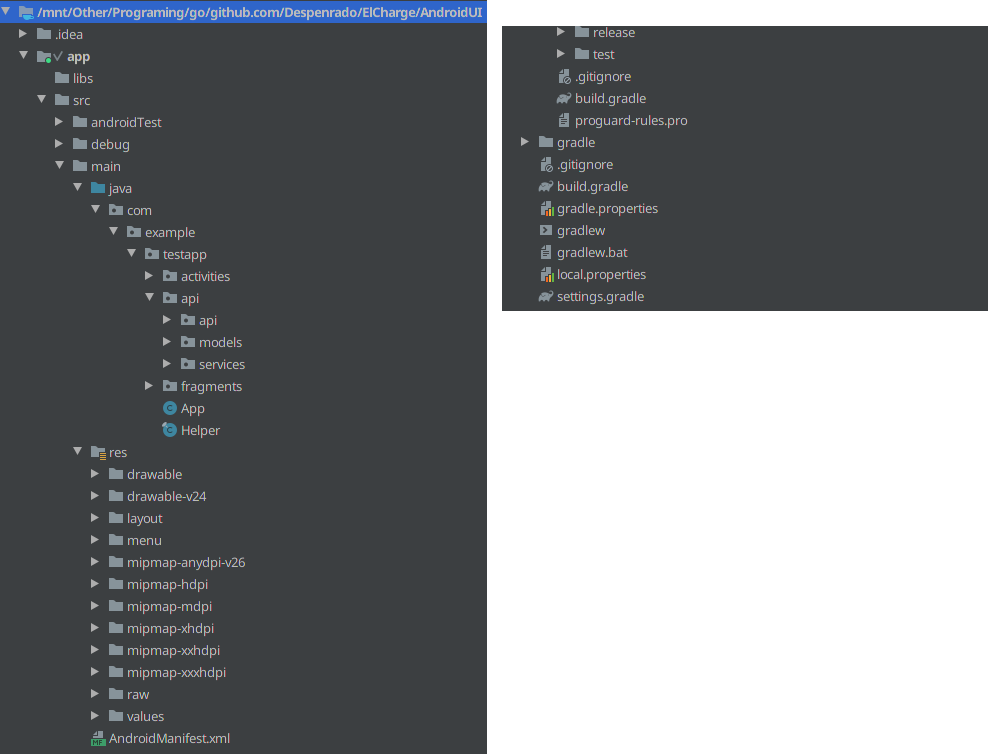
\includegraphics[width=0.4\linewidth]{rys03/frontend_file_struct.png}
\caption{Struktura plików aplikacji mobilnej}
\label{fig:frontend_file_structure}
\end{figure}

Zawartość znaczących katalogów i plików:
\begin{itemize}
    \item katalog \texttt{main/java/com/example/testapp/activities} zawiera klasy \texttt{activity}, są ekranami aplikacji, na których umieszczone wszystkie komponenty interfejsu użytkownika.
    \item katalog \texttt{main/java/com/example/testapp/api} zawiera modeli danych (\texttt{katalog models}), sposób komunikacji (katalog \texttt{services}) oraz endpointy (katalog \texttt{api} na rysunku \ref{fig:frontend_file_structure_1}a) do komunikacji z częścią serwerową .
    \item katalog \texttt{main/java/com/example/testapp/fragments} zawiera klasy fragmentów (rys. \ref{fig:frontend_file_structure_1}b), które umieszczają się w kontenerze na \texttt{activity} i zawierają elementy interfejsu użytkownika (przyciski, pola tekstowe i inne).
    \item w katalogu \texttt{res} znajdują się zasoby aplikacji, na przykład: plik konfiguracyjny (\texttt{res/raw/config.properties}), opisy komponentów oraz ich dyslokacja na fragmentach i oknach aplikacji (\texttt{res/layout/} na rysunku \ref{fig:frontend_file_structure_1}c) i inne.
    \item plik \texttt{main/androidManifest.xml} (listing \ref{list:androidManifest}) zawiera informację niezbędną do budowy aplikacji: definiowanie \texttt{activity}, uprawnień, klasy podstawowej.
    \item plik \texttt{main/java/com/example/testapp/App.java} jest klasą podstawową, który jest niezbędny do podtrzymywania globalnego stanu aplikacji (\texttt{ApplicatioContext}).
\end{itemize}
\begin{figure}[ht]
	\centering
    \begin{tabular}{@{}rl@{\hspace{3mm}}rl@{\hspace{3mm}}rl@{}}
        a) & \vtop{\vskip-2ex\hbox{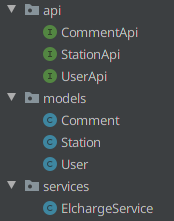
\includegraphics[width=0.253\linewidth]{rys03/frontend_file_struct_api.png}}} &
        b) & \vtop{\vskip-2ex\hbox{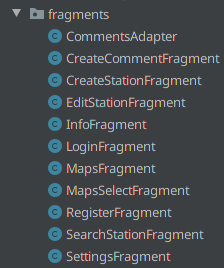
\includegraphics[width=0.27\linewidth]{rys03/frontend_file_struct_fragements.png}}} &
        c) & \vtop{\vskip-2ex\hbox{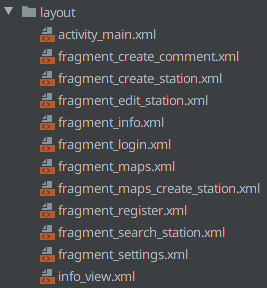
\includegraphics[width=0.30\linewidth]{rys03/frontend_file_struct_layout.png}}}
    \end{tabular}
    \caption{Struktura plików: a) API do połączenia z serwerem, b) klasy fragmentów, c) opis fragmentów.}
    \label{fig:frontend_file_structure_1}
\end{figure}
\begin{lstlisting}[label=list:androidManifest,caption=androidManifest.xml,basicstyle=\tiny\ttfamily]
    <?xml version="1.0" encoding="utf-8"?>
    <manifest xmlns:android="http://schemas.android.com/apk/res/android"
        package="com.example.testapp">
    
        <uses-permission android:name="android.permission.ACCESS_FINE_LOCATION" />
        <uses-permission android:name="android.permission.ACCESS_COARSE_LOCATION" />
        <uses-permission android:name="android.permission.INTERNET" />
        <uses-permission android:name="android.permission.ACCESS_NETWORK_STATE" />
        <uses-permission android:name="android.permission.READ_EXTERNAL_STORAGE" />
        <uses-permission android:name="android.permission.WRITE_EXTERNAL_STORAGE"/>
    
        <application
            android:name=".App"
            android:allowBackup="true"
            android:icon="@mipmap/ic_launcher"
            android:label="@string/app_name"
            android:roundIcon="@mipmap/ic_launcher_round"
            android:supportsRtl="true"
            android:theme="@style/AppTheme"
            android:usesCleartextTraffic="true">
            <meta-data
                android:name="com.google.android.geo.API_KEY"
                android:value="@string/google_maps_key" />
    
            <activity android:name=".activities.MainActivity">
                <intent-filter>
                    <action android:name="android.intent.action.MAIN" />
    
                    <category android:name="android.intent.category.LAUNCHER" />
                </intent-filter>
            </activity>
        </application>
    
    </manifest>
\end{lstlisting}

 
\paragraph{Modele danych:} \texttt{User} (listing \ref{list:user_class}), \texttt{Station} (listing \ref{list:station_class}), \texttt{Comment} (listing \ref{list:comment_class}). W listingach komentarz \texttt{// GETTERS and SETTERS} pokazuje, że w kodzie programu tym miejscu znajdują się proste metody do zapisu i wczytania pól klasy.
Adnotacja \texttt{@SerializedName} ustala nazwę do dekodowania do formatu JSON i na odwrót.

% TO DO: za dużo listingów !!!!! Wystarczy pokazać przykład mapowania na jednym modelu, a potem powiedzieć, że dla pozostałych jest podobnie.
% TO DO: UWAGA POWYŻEJ NIE ZOSTAŁA UWZGLĘNIONA
% TO DO: Powtarzam: w pracy jest za dużo listingów. Nie można przcież kopiować całego kodu!!!!! Wystarczy napisać, że zamodelowano takie a takie klasy, że na listingu pokazano klasę przyładową (np. User). Można też pokazać diagram klas UML z wszystkimi klasami. !!!!!

\begin{lstlisting}[label=list:user_class,caption=Plik \texttt{main/java/com/example/testapp/api/api/UserApi.java},basicstyle=\tiny\ttfamily]
    public class User {
        @SerializedName("_id")
        private String id;
        @SerializedName("user_name")
        private String userName;
        @SerializedName("email")
        private String email;
        @SerializedName("password")
        private String password;
        @SerializedName("update_at")
        private String updateAt;
    
        public User() {
        }
    
        public User(String id, String userName, String email, String password, String updateAt) {
            this.id = id;
            this.userName = userName;
            this.email = email;
            this.password = password;
            this.updateAt = updateAt;
        }
        // GETTERS and SETTERS
    }
\end{lstlisting}

%%%\begin{lstlisting}[label=list:station_class,caption=Plik \texttt{main/java/com/example/testapp/api/api/StationApi.java},basicstyle=\tiny\ttfamily]
    %%%public class Station {
        %%%@SerializedName("_id")
        %%%private String id;
        %%%@SerializedName("owner_id")
        %%%private String ownerID;
        %%%@SerializedName("description")
        %%%private String description;
        %%%@SerializedName("station_name")
        %%%private String stationName;
        %%%@SerializedName("latitude")
        %%%private double latitude;
        %%%@SerializedName("longitude")
        %%%private double longitude;
        %%%@SerializedName("update_at")
        %%%private String updateAt;
        %%%@SerializedName("rating")
        %%%private float rating;
        %%%@SerializedName("comments")
        %%%private ArrayList<Comment> comments;
    %%%
        %%%public Station() {
        %%%}
    %%%
        %%%public Station(String id, String ownerID, String description, String stationName, double latitude, double longitude, String updateAt, float rating, ArrayList<Comment> comments) {
            %%%this.id = id;
            %%%this.ownerID = ownerID;
            %%%this.description = description;
            %%%this.stationName = stationName;
            %%%this.latitude = latitude;
            %%%this.longitude = longitude;
            %%%this.updateAt = updateAt;
            %%%this.rating = rating;
            %%%this.comments = comments;
        %%%}
        %%%// GETTERS and SETTERS
    %%%}
%%%\end{lstlisting}
%%%
%%%\begin{lstlisting}[label=list:comment_class,caption=Plik \texttt{main/java/com/example/testapp/api/api/CommentApi.java},basicstyle=\tiny\ttfamily]
    %%%public class Comment {
        %%%@SerializedName("_id")
        %%%private String id;
        %%%@SerializedName("user_id")
        %%%private String userID;
        %%%@SerializedName("user_name")
        %%%private String userName;
        %%%@SerializedName("text")
        %%%private String text;
        %%%@SerializedName("rating")
        %%%private float rating;
        %%%@SerializedName("create_at")
        %%%private String createAt;
        %%%@SerializedName("update_at")
        %%%private String updateAt;
    %%%
        %%%public Comment() {
        %%%}
    %%%
        %%%public Comment(String id, String userID, String userName, String text, float raiting, String createAt, String updateAt) {
            %%%this.id = id;
            %%%this.userID = userID;
            %%%this.userName = userName;
            %%%this.text = text;
            %%%this.rating = raiting;
            %%%this.createAt = createAt;
            %%%this.updateAt = updateAt;
        %%%}
        %%%// GETTERS and SETTERS
    %%%}
%%%\end{lstlisting}

\paragraph{API:} 
Zaimplementowane API podzielono na trzy części: \texttt{UserApi}, % (listing \ref{list:android_api_user}), 
\texttt{StationApi}, % (listing \ref{list:android_api_station}), 
\texttt{CommentApi}. %(listing \ref{list:android_api_comment}) 
Metody API służą do komunikacji z częścią serwerową.

Zastosowany framework pozwala na zadeklarowanie metod protokołu HTTP  \texttt{POST}, \texttt{PUT}, \texttt{GET}, \texttt{DELETE} obsługiwanych w danej metodzie interfejsu na danym adresie URL poprzez zastosowanie adnotacji. Adnotacja \texttt{Body} pozwala na zadeklarowanie zamieszczenia danych w ciele zapytania. Adnotacja \texttt{Path} mówi, że dane ukryte są w adresie URL. Adnotacja \texttt{Query} mówi, że dane przekazane są jako parametry w adresie URL. Na listingu~\ref{list:android_api_user} pokazano przykład implementacji \texttt{UserAPI}.

\begin{lstlisting}[label=list:android_api_user,caption=Plik \texttt{main/java/com/example/testapp/api/api/UserApi.java},basicstyle=\tiny\ttfamily]
    public interface UserApi {
        @POST("users")
        public Single<Response<User>> createUser(@Body User body);
    
        @POST("login")
        public Single<Response<User>> login(@Body User body);
    
        @GET("logout/{id}")
        public Single<ResponseBody> logout(@Path("id") String id);
    }
\end{lstlisting}

% TO DO: proszę stworzyć tabelkę z opisem api: metoda http, endpoint(url), opis

%%%\begin{lstlisting}[label=list:android_api_station,caption=Plik \texttt{main/java/com/example/testapp/api/api/StationApi.java},basicstyle=\tiny\ttfamily]
    %%%public interface StationApi {
%%%
        %%%@POST("stations")
        %%%public Single<Response<Station>> createStation(@Body Station station);
    %%%
        %%%@GET("stations/read")
        %%%public Single<Response<List<Station>>> readStationsByLatAndLngAndDist(@Query("skip") int skip, @Query("limit") int limit, @Query("lat") double lat, @Query("lng") double lng, @Query("dist") int dist);
    %%%
        %%%@GET("stations/read")
        %%%public Single<Response<Station>> readStationsByLatAndLng(@Query("skip") int skip, @Query("limit") int limit, @Query("lat") double lat, @Query("lng") double lng);
    %%%
        %%%@GET("stations/read")
        %%%public Single<Response<List<Station>>> readStationsByDescription(@Query("skip") int skip, @Query("limit") int limit, @Query("descr") String descr);
    %%%
        %%%@GET("stations/read")
        %%%public Single<Response<List<Station>>> readStationsByName(@Query("skip") int skip, @Query("limit") int limit, @Query("name") String name);
    %%%
        %%%@GET("stations/read")
        %%%public Single<Response<List<Station>>> readStations(@Query("skip") int skip, @Query("limit") int limit);
    %%%
        %%%@GET("stations/{id}")
        %%%public Single<Response<Station>> findById(@Path("id") String id);
    %%%
        %%%@PUT("stations/{id}")
        %%%public Single<Response<Station>> updateById(@Path("id") String id, @Query("ownid") String ownid, @Body Station station);
    %%%
        %%%@DELETE("stations/{id}")
        %%%public Single<ResponseBody> deleteById(@Path("id") String id);
    %%%}
%%%\end{lstlisting}
%%%
%%%\begin{lstlisting}[label=list:android_api_comment,caption=Plik \texttt{main/java/com/example/testapp/api/api/CommentApi.java},basicstyle=\tiny\ttfamily]
    %%%public interface CommentApi {
        %%%@POST("stations/\{sid\}/comments")
        %%%public Single<Response<Comment>> createComment(@Path("sid") String sid, @Body Comment comment);
    %%%
        %%%@GET("stations/\{sid\}/comments/read")
        %%%public Single<Response<List<Comment>>> readComments(@Path("sid") String sid, @Query("skip") int skip, @Query("limit") int limit);
    %%%
        %%%@GET("stations/\{sid\}/comments/{id}")
        %%%public Single<Response<Comment>> findById(@Path("sid") String sid, @Path("id") String id);
    %%%
        %%%@PUT("stations/\{sid\}/comments/{id}")
        %%%public Single<Response<Comment>> updateById(@Path("sid") String sid, @Path("id") String id, @Body Comment comment);
    %%%
        %%%@DELETE("stations/\{sid\}/comments/{id}")
        %%%public Single<ResponseBody> deleteById(@Path("sid") String sid, @Path("id") String id);
    %%%}
%%%\end{lstlisting}

\subsubsection{Komunikacja z częścią serwerową}
Sposób komunikacji z częścią serwerową oraz etapy pośrednicze (zostały zdefiniowane w metodzie \texttt{createOkHttpClient()}), w których zachodzi dodawanie nagłówka oraz pisanie logów zapytań i odpowiedzi, został opisany w klasie \texttt{ElchargeService} (listing \ref{list:android_elchargeservice}). Został użyty HTTP klient \texttt{OkHttp3} oraz jego opakowanie \texttt{Retrofit2}.
\begin{lstlisting}[label=list:android_elchargeservice,caption=obsługa komunikacji z częścią serwerową,basicstyle=\tiny\ttfamily]
    public class ElchargeService {
    String apiAddr;
    String token;
    UserApi userApi;
    StationApi stationApi;
    CommentApi commentApi;
    User user;

    public ElchargeService(){
        apiAddr = Helper.getConfigValue(App.getAppContext(),"apiserver_addr");
        token = Helper.getConfigValue(App.getAppContext(),"apiserver_token");
        Retrofit retrofit = createRetrofit();
        userApi = retrofit.create(UserApi.class);
        stationApi = retrofit.create(StationApi.class);
        commentApi = retrofit.create(CommentApi.class);
    }

    private OkHttpClient createOkHttpClient() {
        OkHttpClient.Builder httpClient = new OkHttpClient.Builder();
        httpClient.addInterceptor(new Interceptor() {
            @Override
            public Response intercept( Chain chain) throws IOException {
                Request request = chain.request().newBuilder()
                        .addHeader("Authorization", token)
                        .build();
                return chain.proceed(request);
            }
        });
        HttpLoggingInterceptor logging = new HttpLoggingInterceptor();
        logging.setLevel(HttpLoggingInterceptor.Level.BODY);
        httpClient.addInterceptor(logging);
        return httpClient.build();
    }

    private Retrofit createRetrofit() {
        return new Retrofit.Builder()
                .baseUrl(apiAddr)
                .client(createOkHttpClient())
                .addCallAdapterFactory(RxJava2CallAdapterFactory.create())
                .addConverterFactory(GsonConverterFactory.create())
                .build();
    }

    public void setToken(String token) {
        Helper.setConfigValue(App.getAppContext(),"apiserver_token", token);
        this.token = token;
    }

    // GETTERS and SETTERS
}
\end{lstlisting}

\label{text:android_api_service}
Komunikacja z serwerem w celu zwiększenia pozytywnego doświadczenia pracy użytkownika z aplikacją zrobiona w sposób asynchroniczny za pomocą biblioteki \texttt{RxJava2}.
Do serwera wysyła się zapytanie na adres URL za pomocą odpowiedniego interfejsu API, indujących się w katalogu \texttt{main/java/com/example/testapp/api/api} (listingi tych klas: \ref{list:android_api_user}, \ref{list:android_api_station}, \ref{list:android_api_comment}).
Dałej zachodzi oczekiwanie na odpowiedź (\texttt{subscribeOn(Shedulers.io())}), po otrzymaniu odpowiedzi w głównym wątku aplikacji (\texttt{observeON(AndroidShedulers.mainThread)}) wykonuje się kod opisany poprzez realizację klasy abstrakcyjnej \texttt{DisposableSingleObserver<T>}. Podczas realizacji tej klasy należy przedefiniować metodę \texttt{onSucces(Object)} (opis działań przy otrzymaniu odpowiedzi od serwera) oraz \texttt{onError(Throwable)} (opis działań przy braku odpowiedzi od serwera).
Przykład kody na podstawie logowania znajduje się w listingu \ref{list:android_login_async}. Przy zamknięciu fragmentu lub aplikacji przez użytkownika, kanał oczekujący na odpowiedź z serwera będzie również zamknięty.
\subsubsection{Układ interfejsu graficznego}
Ekran aplikacji składa się z kilku warstw:
\begin{itemize}
    \item \texttt{Activity} to samodzielny ekran, na którym umieszczają się inne elementy (warstwy, przyciski, teksty i inne).
    \item \texttt{Fragment} to ekran, na którym umieszczają się inne elementy (warstwy, przyciski, teksty i inne). Nie jest samodzielnym ekranem. Zwykle umieszcza się w kontenerze.
\end{itemize}

Dla umieszczania oraz definiowania elementów na ekranie wykorzystane opisy w postaci plików \texttt{xml} (ang. \textit{eXtensible Markup Language}), które przechowywane w katalogu \texttt{main/res}. Na listingu \ref{list:android_xml_create_comment} przedstawiony plik \texttt{main/res/layout/fragment\_create\_comment.xml}.
Jest to opis fragmentu tworzenia nowego komentarza (rys. \ref{fig:front_comment_create}). Aplikacja korzysta z jednego ekranu \texttt{Activity} na którym na dole znajduje się menu. Natomiast pozostałą, większą, przestrzeń ekranu zajmuje kontener do fragmentu, na fragmentach umieszczają się różne elementy aplikacji (przyciski, teksty i inne).
Takie podejście pozwala nakładać fragmenty jeden na jednego, dla uniknięcia usunięcia już wprowadzonej informacji przez użytkownika, oraz usuwać już niepotrzebne. Opisy zachowania elementów ekranu znajdują się w odpowiednich klasach opisujących zachowanie całego ekranu i elementów na nim. Te klasy napisane w języku Java (pliki w katalogu \texttt{main/java/com/example/testapp/fragments}) (przykład w listingu \ref{list:CreateCommentFragment}).
% Przepraszam za te wielkie listigi, ale to najmniejsze. musiałem pokazać jak wyglądają te pliki
\begin{lstlisting}[label=list:android_xml_create_comment,caption=Opis fragmentu tworzenia komentarza,basicstyle=\tiny\ttfamily]
    <?xml version="1.0" encoding="utf-8"?>
    <androidx.constraintlayout.widget.ConstraintLayout xmlns:android="http://schemas.android.com/apk/res/android"
        xmlns:app="http://schemas.android.com/apk/res-auto"
        xmlns:tools="http://schemas.android.com/tools"
        android:layout_width="match_parent"
        android:layout_height="match_parent"
        android:background="@color/cardview_light_background"
        tools:context=".fragments.CreateCommentFragment">
    
        <EditText
            android:id="@+id/editTextText"
            android:layout_width="0dp"
            android:layout_height="0dp"
            android:layout_marginStart="16dp"
            android:layout_marginEnd="16dp"
            android:layout_marginBottom="505dp"
            android:ems="10"
            android:hint="Text"
            android:maxLength="512"
            app:layout_constraintBottom_toBottomOf="parent"
            app:layout_constraintEnd_toEndOf="parent"
            app:layout_constraintStart_toStartOf="parent"
            app:layout_constraintTop_toBottomOf="@+id/ratingBar" />
    
        <RatingBar
            android:id="@+id/ratingBar"
            android:layout_width="wrap_content"
            android:layout_height="wrap_content"
            android:layout_marginStart="72dp"
            android:layout_marginTop="26dp"
            android:layout_marginEnd="73dp"
            android:layout_marginBottom="22dp"
            android:backgroundTint="#2ED573"
            android:numStars="5"
            android:stepSize=".5"
            app:layout_constraintBottom_toTopOf="@+id/editTextText"
            app:layout_constraintEnd_toEndOf="@+id/editTextText"
            app:layout_constraintStart_toStartOf="parent"
            app:layout_constraintTop_toTopOf="parent" />
    
        <Button
            android:id="@+id/buttonSave"
            android:layout_width="wrap_content"
            android:layout_height="wrap_content"
            android:layout_marginTop="136dp"
            android:layout_marginEnd="76dp"
            android:text="Save"
            app:layout_constraintEnd_toEndOf="parent"
            app:layout_constraintTop_toBottomOf="@+id/editTextText" />
    
        <Button
            android:id="@+id/buttonCancel"
            android:layout_width="wrap_content"
            android:layout_height="wrap_content"
            android:layout_marginStart="76dp"
            android:layout_marginTop="136dp"
            android:text="cancel"
            app:layout_constraintStart_toStartOf="parent"
            app:layout_constraintTop_toBottomOf="@+id/editTextText" />
    </androidx.constraintlayout.widget.ConstraintLayout>
\end{lstlisting}
\begin{lstlisting}[label=list:CreateCommentFragment,caption=Klasa opisująca zachowanie elementów na fragemencie tworzenia komentarza,basicstyle=\tiny\ttfamily]
    public class CreateCommentFragment extends Fragment {

        private CompositeDisposable disposable = new CompositeDisposable();
        private App app;
        private String stationID;
    
        public CreateCommentFragment(String stationID) {
            this.stationID = stationID;
        }
    
        @Override
        public void onCreate(Bundle savedInstanceState) {
            super.onCreate(savedInstanceState);
        }
    
        @Override
        public View onCreateView(LayoutInflater inflater, ViewGroup container,
                                 Bundle savedInstanceState) {
            return inflater.inflate(R.layout.fragment_create_comment, container, false);
        }
    
        @Override
        public void onViewCreated(@NonNull View view, @Nullable Bundle savedInstanceState) {
            super.onViewCreated(view, savedInstanceState);
            this.app = (App) getActivity().getApplication();
            Button btnSave = (Button)getView().findViewById(R.id.buttonSave);
            btnSave.setOnClickListener(this::onButtonSave);
            Button btnCancel = (Button)getView().findViewById(R.id.buttonCancel);
            btnCancel.setOnClickListener(this::onButtonCancel);
        }
    
        private void onButtonSave(View v){
            Comment comment = new Comment();
            comment.setRating(((RatingBar)getView().findViewById(R.id.ratingBar)).getRating());
            comment.setText(((EditText)getView().findViewById(R.id.editTextText)).getText().toString());
            comment.setUserID(app.getElchargeService().getUser().getId());
            comment.setUserName(app.getElchargeService().getUser().getUserName());
            createComment(comment);
        }
    
        private void onButtonCancel(View v){
            getFragmentManager().beginTransaction().remove(this).commit();
        }
    }
\end{lstlisting}

\subsection{Funkcje aplikacji mobilnej}
W tej sekcji opisano współdziałanie użytkownika i systemu oraz implementacja tych części.

\subsubsection{Logowanie i rejestracja}
Dla otwarcia strony logowania lub rejestracji można nacisnąć odpowiedni przycisk, który znajduje się w prawym dolnym rogu (koło zębate). Otworzą się ustalenia jak na rysunku \ref{fig:frontend_settings}a. Na tym fragmencie można zalogować się (przycisk \texttt{Log in}) lub wylogować się (przycisk \texttt{Log out}).
Przy próbie wykorzystania elementów aplikacji, które potrzebują autentykacji, ale użytkownik jeszcze nie będzie zalogowany do systemu, logowanie (rys. \ref{fig:frontend_settings}b) będzie proponowane automatycznie. Ze strony logowania można trafić do strony rejestracji (rys. \ref{fig:frontend_settings}c) za pomocą odpowiedniego przycisku.
Jeśli logowanie zostało proponowane automatycznie, dane poprzedniego ekranu nie będą usuwane, więc po zalogowaniu lub rejestracji można kontynuować pracę.

\begin{figure}[ht]
	\centering
    \begin{tabular}{@{}rl@{\hspace{3mm}}rl@{\hspace{3mm}}rl@{}}
        a) & \vtop{\vskip-2ex\hbox{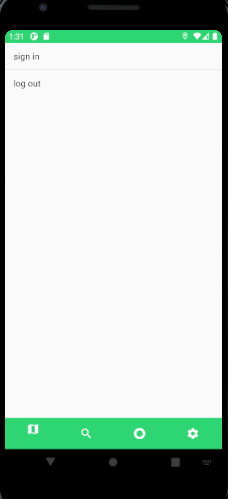
\includegraphics[width=0.25\linewidth]{rys03/front_settings.png}}} &
        b) & \vtop{\vskip-2ex\hbox{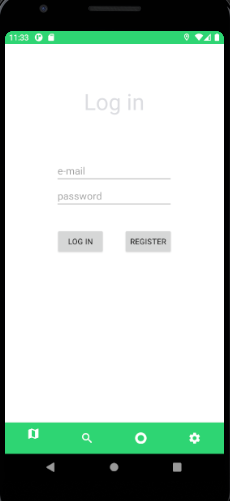
\includegraphics[width=0.25\linewidth]{rys03/front_login.png}}} &
        c) & \vtop{\vskip-2ex\hbox{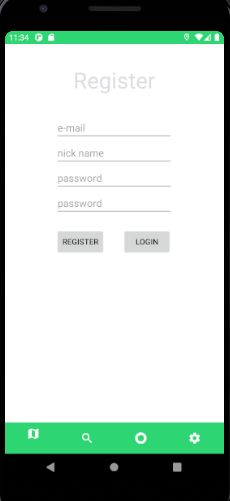
\includegraphics[width=0.25\linewidth]{rys03/front_register.png}}}
    \end{tabular}
    \caption{Interfejs użytkownika: a) ustawienia, b) logowanie, c) rejestracja.}
    \label{fig:frontend_settings}
\end{figure}

Po \label{text:login} wprowadzeniu danych i wciśnięciu przycisku \texttt{Log in} przez użytkownika na stronie logowania, wszystkie pola muszą być niepuste, wysyła się zapytanie do serwera (opis API połączenia z serwerem \ref{text:android_api_service}) z danymi do logowania (listing \ref{list:android_login_async}). Obsługa przycisku zachodzi w metodzie \texttt{onButtonLoginClick} (listing \ref{list:android_login_check}).
Przy pomyślnym zalogowaniu JTW token zachowuje się w pliku konfiguracyjnym, w celu automatycznego logowania przy następnym wykorzystaniu aplikacji, oraz zamyka się fragment logowania, za pomocą klasy sterującej fragmentami (\texttt{FragmenManager}). Przy otwarciu fragmentu logowania lub rejestracji wcześniejszy fragment pozostaje pracować na dolnej warstwie fragmentów, co pozwala zachowywać wprowadzone dane.
Cała klasa obsługująca znajduje się w pliku \texttt{main/java/com/example/testapp/fragments/LoginFragment.java}.
\begin{lstlisting}[label=list:android_login_check,caption=Obsługa przycisku login,basicstyle=\tiny\ttfamily]
    public void onButtonLoginClick(View v) {
        EditText email = (EditText) getView().findViewById(R.id.editTextEmail);
        EditText pass2 = (EditText) getView().findViewById(R.id.editTextPassword);
        if (email.getText().toString().equals("") || pass2.getText().toString().equals("")) {
            Helper.messageLogger(App.getAppContext(), Helper.LogType.NONE, "login", "Login or Password is incorrect");
        } else {
            User u = new User();
            u.setEmail(email.getText().toString());
            u.setPassword(pass2.getText().toString());
            login(u);
        }
    }
\end{lstlisting}
\begin{lstlisting}[label=list:android_login_async,caption=Logowanie: wysłanie zapytania i obsługa odpowiedzi,basicstyle=\tiny\ttfamily]
    private void login(User user) {
        final LoginFragment tmpcls = this;
        disposable.add(app.getElchargeService().getUserApi().login(user)
                .subscribeOn(Schedulers.io())
                .observeOn(AndroidSchedulers.mainThread())
                .subscribeWith(new DisposableSingleObserver<Response<User>>() {
                    @Override
                    public void onSuccess(Response<User> response) {
                        try {
                            if (response.code() == 200) {
                                User tmp = response.body();
                                String token = response.headers().get("Authorization");
                                app.getElchargeService().setToken(token);
                                app.getElchargeService().setUser(tmp);
                                Helper.messageLogger(App.getAppContext(), Helper.LogType.INFO, "login", "LOGGED IN");
                                getFragmentManager().beginTransaction().remove(tmpcls).commit();
                            } else {
                                Helper.messageLogger(App.getAppContext(), Helper.LogType.INFO, "login", response.message());
                            }

                        } catch (Exception e) {
                            Helper.messageLogger(App.getAppContext(), Helper.LogType.ERR, "login", e.getMessage());
                        }
                    }

                    @Override
                    public void onError(Throwable e) {
                        Helper.messageLogger(App.getAppContext(), Helper.LogType.ERR, "login", e.getMessage());
                    }
                }));
    }
\end{lstlisting}

Rejestracja działa w podobny sposób do logowania (opis: \ref{text:login}): sprawdzanie wprowadzonych przez użytkownika danych oraz komunikacja z częścią serwerową. Cała klasa obsługująca rejestrację znajduje się w pliku \texttt{main/java/com/example/testapp/fragments/RegisterFragment.java}.

\subsubsection{Stacja}
\paragraph{Dodawanie\newline}
Jedną z najważniejszych funkcji jest tworzenie stacji ładowania.
Dla jej tworzenia stworzony fragment aplikacji dostępny pod przyciskiem kółka (trzeci znaczek w menu pod spodem) (rys. \ref{fig:frontend_station_create}a).
Za pomocą przycisku \texttt{MAP} można nie wprowadzać współrzędne ręcznie, a ustalić miejsce na za pomocą mapy (rys. \ref{fig:frontend_station_create}b).
Za pracę ze stroną zawierającą interaktywną mapą odpowiada fragment \texttt{fragment\_maps\_create\_station.xml} oraz kalsa \texttt{MapsSelectFragment}.\begin{figure}[ht]
	\centering
    \begin{tabular}{@{}rl@{\hspace{3mm}}rl@{}}
        a) & \vtop{\vskip-2ex\hbox{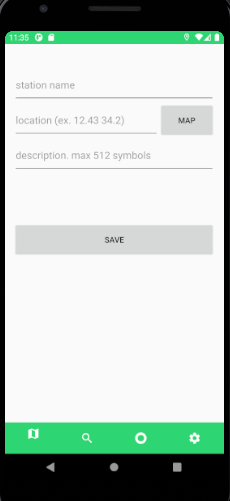
\includegraphics[width=0.3\linewidth]{rys03/front_station_create.png}}} &
        b) & \vtop{\vskip-2ex\hbox{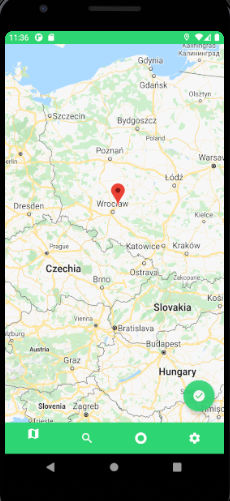
\includegraphics[width=0.3\linewidth]{rys03/front_map_fing.png}}}
    \end{tabular}
    \caption{Interfejs użytkownika: a) tworzenie stacji, b) ustalenie markera na mapie.}
    \label{fig:frontend_station_create}
\end{figure}

Naciśnięcie przycisku \texttt{SAVE} powoduje sprawdzenie wprowadzonych danych oraz wysłanie odpowiedniego zapytania do części serwerowej w celu tworzenia nowego wpisu w bazie danych. Jeśli użytkownik nie został zalogowany lub zarejestrowany, wyświetla się okno logowania lub rejestracji (rys. \ref{fig:frontend_settings}b, \ref{fig:frontend_settings}c).
Klasa obsługująca ten fragment znajduje się w pliku \texttt{main/java/com/example/testapp/fragments/CreateStationFragment.java}.
% TO DO: za dużo listingów kodu !!!!!!
% TO VERIFY

\paragraph{Wyszukiwanie\newline}
Najważniejszą funkcją aplikacji jest wyszukiwanie stacji ładowania do pojazdów elektrycznych. W tym celu został stworzony przycisk w dolnym menu, który wygląda jak lupa (rys. \ref{fig:frontend_station_find}a).
Na tym ekranie można wyszukać stacje ładowania na podstawie: wprowadzonych współrzędnych, ustaleniu miejsca na mapie (rys. \ref{fig:frontend_station_create}b), niniejszej pozycji użytkownika, według części nazwy lub opisu stacji ładowania.
Przy wyszukiwaniu według różnego rodzaju kordynat, istnieje możliwość ustalenia dystansu wyszukiwania za pomocą suwaka.
Naciskając na przycisk \texttt{GO} zalogowany użytkownik trafi na stronę z mapą, gdzie będą oznaczone wyszukane stacje (rys. \ref{fig:frontend_station_find}b).\begin{figure}[ht]
	\centering
    \begin{tabular}{@{}rl@{\hspace{3mm}}rl@{}}
        a) & \vtop{\vskip-2ex\hbox{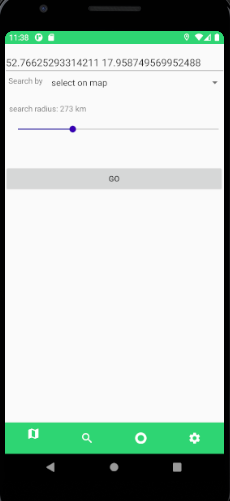
\includegraphics[width=0.3\linewidth]{rys03/front_find.png}}} &
        b) & \vtop{\vskip-2ex\hbox{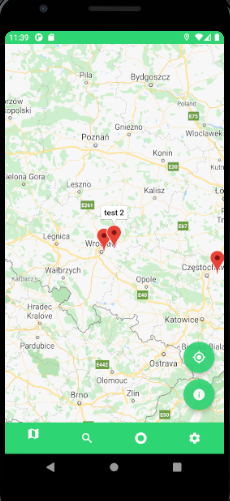
\includegraphics[width=0.3\linewidth]{rys03/front_map_arkers.png}}}
    \end{tabular}
    \caption{Interfejs użytkownika: a) wyszukiwanie stacji, b) lista znalezionych stacji.}
    \label{fig:frontend_station_find}
\end{figure}

W zależności od wybranego, za pomocą spadającego menu, trybu wyszukiwania, będzie wykorzystany odpowiedni API \ref{list:android_api_station}. W przypadku wybory automatycznego wprowadzenia pozycji użytkownika sprawdza się czy aplikacja ma odpowiednie uprawnienia (\texttt{ACCESS\_FINE\_LOCATION, ACCESS\_COARSE\_LOCATION}). Jeśli brak tych uprawnień, odpytuje użytkownika o zezwoleniu na korzystanie z nich.
\texttt{FusedLocationProviderClient} (część SDK Google Mobile Services) pozwala na określenie pozycji nie tylko za pomocą modułu GPS, ale i IP adresie. W przypadku nieudanego otrzymania niniejszej pozycji zostają użyte ostatnie wiadome współrzędne.
Użytkownik też może ustalić marker do wyszukiwania na mapie, wtedy jest wywołany fragment do rysowania mapy (rys. \ref{fig:frontend_station_create}b) i po ustaleniu pozycji, współrzędne będą automatycznie wprowadzone.

\paragraph{Wczytywanie\newline}
Otrzymanie informacji dotyczącej stacji ładowania jest dostępne po wyborze markera na mapie i naciśnięciu przycisku \texttt{info} na tym ekranie (rys. \ref{fig:frontend_station_find}b). Zostanie wysłano zapytanie do serwera z prośbą o zwróceniu informacji dotyczącej wybranej stacji ładowania. Po otrzymaniu odpowiedzi zostanie wyświetlony fragment z nazwą stacji, jej \texttt{id}, opisem, datą ostatniej modyfikacji, oceną, wyliczoną na podstawie komentarzy, i lista komentarzy napisanych do tej stacji w kolejności: najpierw najnowsze.
Komentarze zawierają \texttt{user\_name}, tekst, ocenę oraz datę. Ten fragment jest pokazany na rysunku \ref{fig:frontend_station_info}a.
\begin{figure}[ht]
	\centering
    \begin{tabular}{@{}rl@{\hspace{3mm}}rl@{}}
        a) & \vtop{\vskip-2ex\hbox{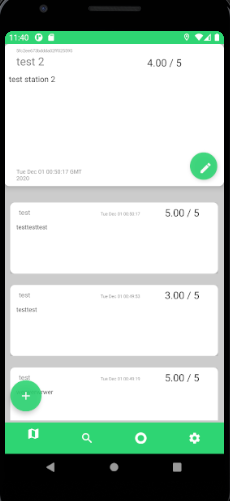
\includegraphics[width=0.3\linewidth]{rys03/front_info.png}}} &
        b) & \vtop{\vskip-2ex\hbox{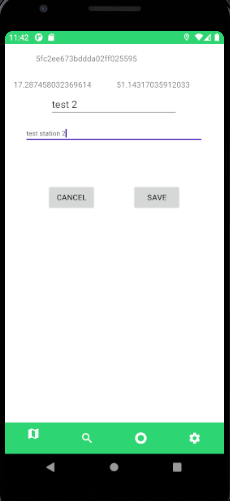
\includegraphics[width=0.3\linewidth]{rys03/front_station_edit.png}}}
    \end{tabular}
    \caption{Interfejs użytkownika: a) wyszukiwanie stacji, b) lista znalezionych stacji.}
    \label{fig:frontend_station_info}
\end{figure}

Do otrzymania aktualnej informacji została zrealizowana metoda \texttt{updateInfo()} w której wysyła się zapytanie do części serwerowej.
Klasa wewnętrzna \texttt{StationDisposableSingleObserver} (listing \ref{list:StationDisposableSingleObserver}), która dziedziczy po klasie abstrakcyjnej \texttt{DisposableSingleObserver}, służy do opracowania i wyświetlania informacji (metoda \texttt{updateInfoOnView()}) na ekranie (listing \ref{list:updateInfoOnView}).
Oczekiwanie na odpowiedź z serwera zachodzi asynchronicznie.
\begin{lstlisting}[label=list:StationDisposableSingleObserver,caption=Wczytanie danych stacji z części serwerowej,basicstyle=\tiny\ttfamily]
    public void updateInfo(){
        disposable.add(app.getElchargeService().getStationApi().readStationsByLatAndLng(0, 0, currentStation.getLatitude(), currentStation.getLongitude())
                .subscribeOn(Schedulers.io())
                .observeOn(AndroidSchedulers.mainThread())
                .subscribeWith(new StationDisposableSingleObserver(this)));
    }

    private class StationDisposableSingleObserver extends DisposableSingleObserver<Response<Station>> {
        private InfoFragment parent;

        public StationDisposableSingleObserver(InfoFragment parent) {
            this.parent = parent;
        }

        @Override
        public void onSuccess(Response<Station> response) {
            try {
                if (response.code() == 200) {
                    Station station = response.body();
                    Helper.messageLogger(App.getAppContext(), Helper.LogType.INFO, "station", Integer.toString(response.code()));
                    currentStation = station;
                    updateInfoOnView();
                } else {
                    Helper.messageLogger(App.getAppContext(), Helper.LogType.INFO, "station", Integer.toString(response.code()));
                    if (response.code() == 401) {
                        LoginFragment lf = new LoginFragment();
                        getFragmentManager().beginTransaction().add(R.id.container, lf).commit();
                        getFragmentManager().beginTransaction().show(lf).commit();
                    }else{
                        getFragmentManager().beginTransaction().remove(parent).commit();
                    }
                }

            } catch (Exception e) {
                Helper.messageLogger(App.getAppContext(), Helper.LogType.ERR, "station", e.getMessage());
            }
        }

        @Override
        public void onError(Throwable e) {
            Helper.messageLogger(App.getAppContext(), Helper.LogType.ERR, "station", e.getMessage());
        }
    }
\end{lstlisting}
\begin{lstlisting}[label=list:updateInfoOnView,caption=Odnowienie informacji o stacji na ekranie,basicstyle=\tiny\ttfamily]
    private void updateInfoOnView(){
        if (app.getElchargeService().getUser().getId().equals(currentStation.getOwnerID())){
            buttonEditStation.show();
        }else {
            buttonEditStation.hide();
        }
        recyclerView = getView().findViewById(R.id.recyclerViewComments);
        recyclerView.setLayoutManager((new LinearLayoutManager(App.getAppContext())));

        commentsAdapter = new CommentsAdapter(currentStation.getComments());
        recyclerView.setAdapter(commentsAdapter);

        ((TextView) getView().findViewById(R.id.stationId)).setText(currentStation.getId());
        ((TextView)getView().findViewById(R.id.stationName)).setText(currentStation.getStationName());
        ((TextView)getView().findViewById(R.id.rating)).setText(String.format("%.2f", currentStation.getRating()) + " / 5");
        ((TextView)getView().findViewById(R.id.description)).setText(currentStation.getDescription());
        ((TextView)getView().findViewById(R.id.date)).setText(Helper.getDateFromISO8601(currentStation.getUpdateAt()));
    }
\end{lstlisting}

\paragraph{Edycja\newline}
Tylko użytkownik, który stworzył stację ładowania do pojazdów elektrycznych, ma możliwość modyfikacji stacji ładowania. Jeśli twórca przegląda swoją stację, obok opisu tej stacji istnieje przycisk (rys. \ref{fig:frontend_station_info}a), za pomocą którego można wejść do strony modyfikacji (rys. \ref{fig:frontend_station_info}b).
Modyfikacji podlegają tylko nazwa i opis. Przycisk \texttt{CANCEL} przewróci na stronę informacji o stacji ładowania. Komunikacja z serwerem zachodzi na tej samej zasadzie, co już opisana wyżej, w części logowania i rejestracji.

\subsubsection{Komentarz}
Komentarzy mogą pisać i przeglądać zalogowane użytkowniki podczas przeglądania informacji o stacji ładowania. Oni są niezbędne do wystawiania oceny stacji.
\paragraph{Dodawanie\newline}
Dodać komentarz można na stronie informacyjnej stacji ładowania (rys. \ref{fig:frontend_station_info}a) za pomocą odpowiedniego przycisku (plus w kółku). Na rysunku \ref{fig:front_comment_create} przedstawiony ekran tworzenia komentarza.
\begin{figure}[ht]
    \centering
    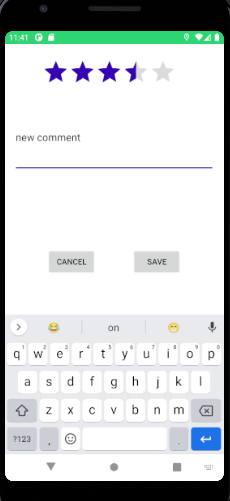
\includegraphics[width=0.25\linewidth]{rys03/front_comment_create.png}
    \caption{Struktura plików}
    \label{fig:front_comment_create}
\end{figure}
Zasada działania jest prosta: walidacja wpisanej informacji, wysłanie zapytania do serwera, asynchroniczne oczekiwanie na odpowiedź, przy udanym tworzeniu — powrót do strony zawierającej informację o stacji ładowania pojazdów elektrycznych.
Użytkownik widzi juz zmieniona informację.